\documentclass[a4paper,12pt]{article}
\usepackage[unicode,verbose]{hyperref}
\usepackage{amsmath,amssymb,amsthm}
\usepackage{pb-diagram}
\usepackage{ucs}
%\usepackage[utf8x]{inputenc}
%\usepackage[russian]{babel}
\usepackage{cmap}
\usepackage{color}
\usepackage[pdftex]{graphicx}
\pagestyle{plain}

%\usepackage{verbatim} 
\newenvironment{comment}
{\par\noindent{\bf TODO}\\}
{\\\hfill$\scriptstyle\blacksquare$\par}

\newtheorem{statement}{Statement}
\theoremstyle{definition} \newtheorem{Def}{Definition}

\begin{document}
\thispagestyle{empty}

\begin{center}
{\Large \bf SAINT-PETERSBURG STATE\\[0.5cm] UNIVERSITY}
\end{center}
\vskip 1 cm
\begin{flushright}
{\large \bf SPbU-IP-09-08}
\end{flushright}
\hfill {}
\vskip 1 cm
\begin{center}
{\Huge \bf Recursive algorithms, branching coefficients \\ for affine algebras and applications\\[0.5cm]
}
\end{center}
\vskip 1.0 cm
\begin{center}
{\Large \bf
Vladimir Lyakhovsky\\[2mm]
Anton Nazarov}
\end{center}
\vfill
\begin{center}
{\large Department of Theoretical Physics\\
}
\end{center}
\vfill
\begin{center}
SAINT-PETERSBURG \\
2009
\end{center}

\newpage

\pagenumbering{arabic}
\title{\textbf{{\Large {Recursive algorithms, branching coefficients affine algebras and applications}}}}
\author{Vladimir Lyakhovsky \thanks{ Supported by
 RFFI grant N 09-01-00504 and the National Project RNP.2.1.1./1575 }\\
Theoretical Department, SPb State University,\\
198904, Sankt-Petersburg, Russia \\
e-mail:lyakh1507@nm.ru \\
[5mm] Anton Nazarov \thanks{ Supported by
the National Project RNP.2.1.1./1575 }\\
Theoretical Department, SPb State University,\\
198904, Sankt-Petersburg, Russia \\
e-mail:antonnaz@gmail.com
}
\maketitle

\begin{abstract}
  Recurrent relations for branching coefficients in affine Lie algebras highest weight modules are studied. The decomposition algorithm for  integrable highest weight modules reduction based on the injection fan technique is adopted to the situation where the Weyl denominator becomes singular with respect to a reductive  subalgebra. We study some modifications of the injection fan technique and demonstrate that it is possible to define the "subtracted fans" that play the role similar to the original one. The possible applications of subtracted fans in CFT models are considered.
\end{abstract}

\section{Introduction}
\label{sec:introduction}

The problem of reduction of a Lie algebra representation to a  subalgebra is studied for several decades and has various applications in physics. In the context of finite-dimensional algebras it is important for the study of great unification models whilst the branching problem for affine Lie algebras emerges in conformal field theory, for example, in the construction of the modular-invariant partition functions \cite{difrancesco1997cft}.

There exist several approaches to the computation of the branching coefficients. Some of them use the BGG
resolution \cite{bernstein1975differential} (for Kac-Moody algebras the algorithm is described in
\cite{kac1990idl},\cite{wakimoto2001idl}), the Schure function series \cite{fauser2006new}, the BRST
cohomology \cite{hwang1994general}, Kac-Peterson formulas \cite{kac1990idl,quella2002branching} or the
combinatorial methods applied in \cite{feigin707principal}.

Usually only the embedding of the maximal reductive subalgebras is considered since the case of non-maximal subalgebra can be obtained using the chain of maximal injections. In this paper we study the recurrent properties for branching coefficients which generalise the recurrent relations obtained earlier (see the paper \cite{ilyin812pbc}and the references therein) to the cases of non-maximal reductive subalgebras. The result is formulated by an introduction of a new injection fan called "subtracted fan". Using this new tools we formulate simple and explicit algorithm for the computation of branching coefficients which is applicable to the non-maximal subalgebras of finite-dimensional and affine Lie algebras.

We show that our algorithm can be used in a study of conformal embeddings where the central charge of the conformal field theory is preserved, and the computations are simplified by taking into account some  physical limitations.

The paper is organised as follows. In the next subsection  we fix the notations used throughout the paper. In the Section \ref{sec:recurr-form-branch} we derive the subtracted recurrent formula for anomalous branching coefficients and describe the decomposition algorithm for integrable highest weight modules of algebra $\mathfrak{g}$ with respect to a reductive subalgebra $\mathfrak{a}$ (subsection \ref{sec:algorithm}). In the next Section \ref{sec:examples} we present several examples and discuss some applications in CFT models (s. \ref{sec:phys-appl}). We conclude the paper with a review of obtained results. Possible future developments are discussed (s. \ref{sec:conclusion}).

\subsection{Notation}
\label{sec:notation}

Consider affine Lie algebras $\frak{g}$ and $\frak{a}$ with the
underlying finite-dimensional subalgebras $\overset{\circ }{\frak{g}}$ and $%
\overset{\circ }{\frak{a}}$ and an injection $\frak{a}\longrightarrow \frak{g%
}$ such that $\frak{a}$ is a reductive subalgebra $\frak{a\subset g}$ with
correlated root spaces: $\frak{h}_{\frak{a}}^{\ast }\subset \frak{h}_{\frak{g%
}}^{\ast }$ and $\frak{h}_{\overset{\circ }{\frak{a}}}^{\ast }\subset \frak{h%
}_{\overset{\circ }{\frak{g}}}^{\ast }$\ .

We use the following notations adopted from the paper \cite{ilyin812pbc}.

$L^{\mu }$\ $\left( L_{\frak{a}}^{\nu }\right) $\ --- the integrable module
of $\frak{g}$ with the highest weight $\mu $\ ; (resp. integrable $\frak{a}$
-module with the highest weight $\nu $ );

$r$ , $\left( r_{\frak{a}}\right) $ --- the rank of the algebra $\frak{g}$ $%
\left( \text{resp. }\frak{a}\right) $ ;

$\Delta $ $\left( \Delta _{\frak{a}}\right) $--- the root system; $\Delta
^{+} $ $\left( \text{resp. }\Delta _{\frak{a}}^{+}\right) $--- the positive
root system (of $\frak{g}$ and $\frak{a}$ respectively);

$\mathrm{mult}\left( \alpha \right) $ $\left( \mathrm{mult}_{\frak{a}}\left(
\alpha \right) \right) $ --- the multiplicity of the root $\alpha$ in $\Delta
$ (resp. in $\left( \Delta _{\frak{a}}\right) $);

$\overset{\circ }{\Delta }$ , $\left( \overset{\circ }{\Delta _{\frak{a}}}%
\right) $ --- the finite root system of the subalgebra $\overset{\circ }{%
\frak{g}}$ (resp. $\overset{\circ }{\frak{a}}$);
$\Theta$, $(\Theta_{\mathfrak{a}})$ --- the highest root of the algebra $\mathfrak{g}$ (resp. subalgebra $\mathfrak{a}$);

$\mathcal{N}^{\mu }$ , $\left( \mathcal{N}_{\frak{a}}^{\nu }\right) $ --- the
weight diagram of $L^{\mu }$ $\left( \text{resp. }L_{\frak{a}}^{\nu }\right)
$ ;

$W$ , $\left( W_{\frak{a}}\right) $--- the corresponding Weyl group;

$C$ , $\left( C_{\frak{a}}\right) $--- the fundamental Weyl chamber;

$\bar{C}, \left(\bar{C_{\mathfrak{a}}}\right)$ --- the closure of the fundamental Weyl chamber;

$\rho $\ , $\left( \rho _{\frak{a}}\right) $\ --- the Weyl vector;

$\epsilon \left( w\right) :=\det \left( w\right) $ ;

$\alpha _{i}$ , $\left( \alpha _{\left( \frak{a}\right) j}\right) $ --- the $i
$-th (resp. $j$-th) basic root for $\frak{g}$ $\left( \text{resp. }\frak{a}%
\right) $; $i=0,\ldots ,r$ ,\ \ $\left( j=0,\ldots ,r_{\frak{a}}\right) $;

$\delta $ --- the imaginary root of $\frak{g}$ (and of $\frak{a}$ if any);

$\alpha _{i}^{\vee }$ , $\left( \alpha _{\left( \frak{a}\right) j}^{\vee
}\right) $--- the basic coroot for $\frak{g}$ $\left( \text{resp. }\frak{a}%
\right) $ , $i=0,\ldots ,r$ ;\ \ $\left( j=0,\ldots ,r_{\frak{a}}\right) $;

$\overset{\circ }{\xi }$ , $\overset{\circ }{\xi _{\left( \frak{a}\right) }}$
--- the finite (classical) part of the weight $\xi \in P$ , $\left( \text{%
resp. }\xi _{\left( \frak{a}\right) }\in P_{\frak{a}}\right) $;

$\lambda =\left( \overset{\circ }{\lambda };k;n\right) $ --- the
decomposition of an affine weight indicating the finite part $\overset{\circ
}{\lambda }$, level $k$ and grade $n$\ .

$P$ $\left( \text{resp. } P_{\frak{a}}\right) $ \ --- the weight lattice;

$M \left( \text{resp. }M_{\frak{a}}\right) :=$

\noindent $=\left\{
\begin{array}{c}
\sum_{i=1}^{r}\mathbf{Z}\alpha _{i}^{\vee }\text{ }\left( \text{resp. }%
\sum_{i=1}^{r}\mathbf{Z}\alpha _{\left( \frak{a}\right) i}^{\vee }\right)
\text{for untwisted algebras or }A_{2r}^{\left( 2\right) }, \\
\sum_{i=1}^{r}\mathbf{Z}\alpha _{i}\text{ }\left( \text{resp. }\sum_{i=1}^{r}%
\mathbf{Z}\alpha _{\left( \frak{a}\right) i}\right) \text{for }A_{r}^{\left(
u\geq 2\right) }\text{ and }A\neq A_{2r}^{\left( 2\right) },
\end{array}
\right\} ;$
$\Psi ^{\left( \mu \right) }:=\sum\limits_{w\in W}\epsilon (w)e^{w\circ (\mu +\rho )-\rho }$ --- the singular weight element for the $\frak{g}$-module $L^{\mu }$;
$\Psi _{\left( \frak{a}\right) }^{\left( \nu \right) }:=\sum\limits_{w\in W_{\frak{a}}}\epsilon (w)e^{w\circ (\nu +\rho
_{_{\frak{a}}})-\rho _{_{\frak{a}}}}$ --- the corresponding singular weight
element for the $\frak{a}$-module $L_{\frak{a}}^{\nu }$;

$\widehat{\Psi ^{\left( \mu \right) }}$ $\left( \widehat{\Psi _{\left( \frak{%
a}\right) }^{\left( \nu \right) }}\right) $ --- the set of singular weights $%
\xi \in P$ $\left( \text{resp. }\in P_{\frak{a}}\right) $ for the module $%
L^{\mu }$ $\left( \text{resp. }L_{\frak{a}}^{\nu }\right) $ with the
coordinates $\left( \overset{\circ }{\xi },k,n,\epsilon \left( w\left( \xi
\right) \right) \right) \mid _{\xi =w\left( \xi \right) \circ (\mu +\rho
)-\rho },$ (resp. $\left( \overset{\circ }{\xi },k,n,\epsilon \left(
w_{a}\left( \xi \right) \right) \right) \mid _{\xi =w_{a}\left( \xi \right)
\circ (\nu +\rho _{a})-\rho _{a}}$ ), (this set is similar to $P_{\mathrm{%
nice}}^{\prime }\left( \mu \right) $ in \cite{wakimoto2001idl})

$m_{\xi }^{\left( \mu \right) }$ , $\left( m_{\xi }^{\left( \nu \right)
}\right) $ --- the multiplicity of the weight $\xi \in P$ \ $\left( \text{%
resp. }\in P_{\frak{a}}\right) $ in the module $L^{\mu }$ , (resp. $\xi \in
L_{\frak{a}}^{\nu } $);

$ch\left( L^{\mu }\right) $ $\left( \text{resp. }ch\left( L_{\frak{a}}^{\nu
}\right) \right) $--- the formal character of $L^{\mu }$ $\left( \text{resp. }%
L_{\frak{a}}^{\nu }\right) $;

$ch\left( L^{\mu }\right) =\frac{\sum_{w\in W}\epsilon (w)e^{w\circ (\mu
+\rho )-\rho }}{\prod_{\alpha \in \Delta ^{+}}\left( 1-e^{-\alpha }\right) ^{%
\mathrm{{mult}\left( \alpha \right) }}}=\frac{\Psi ^{\left( \mu \right) }}{%
\Psi ^{\left( 0\right) }}$ --- the Weyl-Kac formula.

$R:=\prod_{\alpha \in \Delta ^{+}}\left( 1-e^{-\alpha }\right) ^{\mathrm{{%
mult}\left( \alpha \right) }}=\Psi ^{\left( 0\right) }\quad $

\noindent $\left( \text{resp. }R_{\frak{a}}:=\prod_{\alpha \in \Delta _{%
\frak{a}}^{+}}\left( 1-e^{-\alpha }\right) ^{\mathrm{mult}_{\frak{a}}\mathrm{%
\left( \alpha \right) }}=\Psi _{\frak{a}}^{\left( 0\right) }\right) $--- the
denominator.

$  L_{\frak{g}\downarrow \frak{a}}^{\mu }=\bigoplus\limits_{\nu \in P_{\frak{a}}^{+}}b_{\nu }^{\left( \mu \right) }L_{\frak{a}}^{\nu }$ --- the reduction of the representation;


$b^{(\mu)}_{\nu}$ --- the branching coefficients;

\begin{equation}
  \label{eq:21}
  \sum_{\nu \in \bar{C_{\mathfrak{a}}}}b_{\nu }^{\left( \mu \right) }\Psi _{\left( \frak{%
        a}\right) }^{\left( \nu \right) }=\sum_{\lambda \in P_{\frak{a}}}k_{\lambda
  }^{\left( \mu \right) }e^{\lambda }
\end{equation}

 $k_{\lambda}$ --- the anomalous branching coefficients;

It is important to mention that
\begin{equation}
  \label{eq:20}
  b^{(\mu)}_{\nu}=k^{(\mu)}_{\nu} \; \mbox{for} \; \nu\in \bar{C}_{\mathfrak{a}}
\end{equation}

$x_e=\frac{\left|\pi_{\mathfrak{a}} \Theta\right|}{\left|\Theta_{\mathfrak{a}}\right|}$ --- the embedding index.

\section{Recurrent relation for branching coefficients. Singularities and subtractions}
\label{sec:recurr-form-branch}

Our aim is to demonstrate that despite possible singularities arriving in the Weyl denominator
when it is projected to the subalgebra root space injection fan technique can be properly modified.
The result of such modification is that the generalized recurrent relations for anomalous branching
coefficients \eqref{eq:21} must be reformulated in the following form:
\begin{equation}
  \label{eq:1}
  \begin{array}{c}
      k_{\xi }^{\left( \mu \right) }=-\frac{1}{s\left( \gamma _{0}\right) }\left(
  \sum_{\omega\in W_{\bot}\backslash W} \epsilon(\omega)\; {\rm dim}\left(L^{\pi_{\mathfrak{a}_{\bot}}(\omega(\mu+\rho))-\rho_{\mathfrak{a}_{\bot}}}_{\mathfrak{a}_{\bot}}\right) \delta_{\xi-\gamma_0,\pi_{\mathfrak{a}}(\omega(\mu+\rho)-\rho)}+ \right.\\
\left.
+\sum_{\gamma \in
\Gamma _{\frak{a}\subset \frak{g}}}s\left( \gamma +\gamma _{0}\right) k_{\xi
+\gamma }^{\left( \mu \right) }\right)
  \end{array}
   \end{equation}
Here $\mathfrak{a}_{\bot}$ is the subalgebra described by the roots of $\mathfrak{g}$
orthogonal to the root subsystem of $\mathfrak{a}$, $W_{\bot}$ is the corresponding Weyl group,
$\Gamma_{\mathfrak{a}\subset \mathfrak{g}}$ is the set of weights in the expansion
of the denominator $\prod_{\alpha\in \Delta^{+}\setminus \Delta^{+}_{\mathfrak{a}_{\bot}}}
(1-e^{-\alpha})^{\mathrm{mult}(\alpha)-\mathrm{mult}_{\mathfrak{a}}(\alpha)}$ and $s(\gamma)$
is the coefficient of $e^{\gamma}$ in this expansion.
In the next subsection we study the situation in details and prove the validity of this relation.

In the section \ref{sec:algorithm} we  shall describe the  computational algorithm for  branching coefficients
based on this formula and present some examples.

\subsection{Proof of the recurrent relation}
\label{sec:proof}

Consider the branching of a module $L_{\frak{g}}^{\mu }$ in terms of formal characters and
projection operators $\pi_{\mathfrak{a}}$ that bring the roots of $\mathfrak{g}$ to the
weight subspace of $\mathfrak{a}$:
\begin{equation}
  \label{eq:3}
  L_{\frak{g}\downarrow \frak{a}}^{\mu }=\bigoplus\limits_{\nu \in P_{\frak{a}%
    }^{+}}b_{\nu }^{\left( \mu \right) }L_{\frak{a}}^{\nu }\quad
  \Longrightarrow\quad
  \pi_{\mathfrak{a}}(ch L^{\mu}_{\mathfrak{g}})=
  \sum_{\nu\in P^{+}_{\mathfrak{a}}}b^{(\mu)}_{\nu} ch L^{\nu}_{\mathfrak{a}}
\end{equation}
The Weyl-Kac character formula leads to
the equality
\begin{equation}
  \label{eq:4}
  \pi_{\mathfrak{a}}\left(\frac{\sum_{\omega\in W} \epsilon(\omega) e^{\omega(\mu+\rho)-\rho}}
  {\prod_{\alpha\in\Delta^{+}}(1-e^{-\alpha})^{\mathrm{mult}(\alpha)}}\right) =
  \sum_{\nu\in P^{+}_{\mathfrak{a}}}b^{(\mu)}_{\nu}
  \frac{\sum_{\omega\in W_{\mathfrak{a}}}\epsilon(\omega)
  e^{\omega(\nu+\rho_{\mathfrak{a}})-\rho_{\mathfrak{a}}}}
  {\prod_{\beta\in \Delta_{\mathfrak{a}}^{+}}(1-e^{-\beta})^{\mathrm{mult}_{\mathfrak{a}}(\beta)}}
\end{equation}

It is important to keep in mind that the projection of some of positive roots of
the algebra $\mathfrak{g}$ can be equal to zero. These roots are orthogonal to the
root space of the subalgebra $\mathfrak{a}$ embedded into the root space of the
algebra $\mathfrak{g}$. Let's denote the subset of such roots by $\Delta^{+}_{\bot}
=\left\{\alpha\in\Delta_{\mathfrak{g}}^{+}:
\forall \beta\in \Delta_{\mathfrak{a}}^{+},\; \alpha\bot\beta \right\}$.

Notice that if the set $\Delta^{+}_{\bot}$ is non-empty the Weyl reflections
corresponding to the positive roots of $\Delta^{+}_{\bot}$ generate a subgroup
$W_{\bot}$ of the Weyl group $W$. Consider any two positive roots $\alpha,\;
\beta\in \Delta^{+}_{\bot}$ and the corresponding Weyl reflections
$\omega_{\alpha},\; \omega_{\beta}\in W_{\bot}$.  Since roots of the subalgebra
$\mathfrak{a}$ are invariant under $\omega_{\alpha}, \; \omega_{\beta}$ they
are also invariant under the action of $\omega_{\gamma}=\omega_{\alpha}\cdot \omega_{\beta}$.
So the subgroup $W_{\bot}$ preserves the root system of the subalgebra $\mathfrak{a}$.

Thus we have obtained the root system $\Delta_{\bot}$ which is orthogonal to the root
system $\Delta_{\mathfrak{a}}$ and invariant with respect to  $W_{\bot}$ . This root system
can be considered as the root system of a subalgebra $\mathfrak{a}_{\bot}\subset \mathfrak{g}$.

Now we are to find out when the subset $\Delta^{+}_{\bot}$ is non-empty
and the subgroup $W_{\bot}$ and subalgebra $\mathfrak{a}_{\bot}$ are non-trivial.

If $\mathfrak{a}$ is a maximal regular subalgebra of $\mathfrak{g}$ then
the rank of $\mathfrak{a}$ is equal to the rank of $\mathfrak{g}$ and
it is clear that $\Delta^{+}_{\bot}$ is empty.
On the other hand
non-maximal regular embedding of $\mathfrak{a}$ into $\mathfrak{g}$ can be obtained
through the chain of maximal embeddings
$\mathfrak{a}\subset \mathfrak{p}_1\subset \mathfrak{p}_2\subset\dots \subset \mathfrak{g}$.
The maximal regular embeddings are constructed by the exclusion of one or two roots
from the extended Dynkin diagram of the algebra. Since this process can give us
non-connected Dynkin diagrams we can see which roots are orthogonal to the root
space of non-maximal regular subalgebra $\mathfrak{a}$.

Consider for instance regular the embedding of $A_1\subset B_2$.

The extended Dynkin diagram of $B_2$ is presented in the Figure \ref{fig:B2Dynkin}.
\begin{figure}[ph]
  \centering
  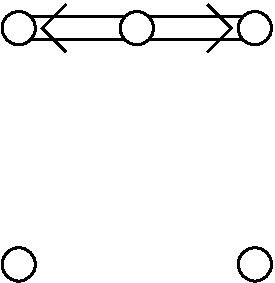
\includegraphics[width=50mm]{B2_A1_diagram.pdf}
  \caption{Extended Dynkin diagram of $B_2$ and embedding of $A_1$}
  \label{fig:B2Dynkin}
\end{figure}
Drop the central node to describe the embedding $A_1\oplus A_1\subset B_2$.
In this case we have: $\mathfrak{a}=A_1$ and $\mathfrak{a}_{\bot}=A_1$.

The simple criterion of $\Delta^{+}_{\bot}$'s non-emptiness for a regular
embedding $\mathfrak{a}\subset \mathfrak{g}$
when both $\mathfrak{a}$ and $\mathfrak{g}$ are simple can be formulated
as follows:
if the Dynkin diagram of $\mathfrak{g}$ can be split into the disconnected
diagrams of $\mathfrak{a}$ and of some subalgebras $\{\mathfrak{\bar{a}}_j\}$
then the subset $\Delta_{\bot}$ is non-empty,
subalgebra $\mathfrak{a}_{\bot}$ is non-trivial and all the
$\mathfrak{\bar{a}}_j$ are the subalgebras of $\mathfrak{a}_{\bot}$.

Note that when we study the regular embedding obtained by dropping the nodes
of the extended Dynkin diagram of the algebra $\mathfrak{g}$ and the
subalgebra $\mathfrak{a}$ is one of the connected components,
the subalgebra $\mathfrak{a}_{\bot}$ may be larger than the algebra
generated by the remaining connected components.
Consider for example the embedding of $B_2\subset B_4$ (the figure \ref{fig:dynkin}).
In this case by eliminating
the simple root $\alpha_2=e_2-e_3$ one splits the extended Dynkin diagram of $B_4$
into the diagrams of the subalgebra $\mathfrak{a}=B_2$ and that of the direct
sum $A_1 \oplus A_1 $. But the subalgebra $\mathfrak{a}_{\bot}$ is equal not to
$A_1\oplus A_1$ but to $B_2$ (the root system of $B_4$ contains not only $\alpha_2=e_2-e_3$ but also $e_2$).

Such effects are due to the fact that the subalgebras $\mathfrak{a}$ and $\mathfrak{a}_{\bot}$ must not form a direct sum in $\mathfrak{g}$.  
Consider the case of such a regular embedding $\mathfrak{a}\subset \mathfrak{g}$ where both algebras are simple and the diagram of the subalgebra $\mathfrak{a}_{\bot}$ is not a subdiagram of the extended Dynkin diagram $\mathfrak{g}$.
 Drop the subdiagram of $\mathfrak{a}$ and the node $\alpha'$ that connects it with all the remaining nodes of the diagram of $\mathfrak{g}$. Consider the remaining diagram. This diagram is the diagram of the algebra $\mathfrak{\bar{a}}$ of $\mathrm{rank}(\mathfrak{\bar{a}}) = \mathrm{rank}(\mathfrak{g})-\mathrm{rank}(\mathfrak{a})$. It is clear that $\mathfrak{\bar{a}}\subset \mathfrak{a}_{\bot}$. So the question is whether $\mathfrak{a}_{\bot}$ has additional roots, which are not the roots of $\mathfrak{\bar{a}}$ but are the linear combinations of them. It is possible when the set of angles between the roots of $\mathfrak{\bar{a}}$ does not contain all the angles between the roots of $\mathfrak{a}$, then reflecting the roots of $\mathfrak{a}$ by $s_{\alpha'}$ we get the additional roots of $\mathfrak{a}_{\bot}$.

All the cases are listed in the table \ref{tab:diagrams}.
\begin{table}[ph]
\label{tab:diagrams}
\noindent  \centering{
\begin{tabular}{|l|l|l|l|}
  \hline
  $\mathfrak{g}$ & Extended diagram of the algebra $\mathfrak{g}$ & Diagrams of the subalgebras $\mathfrak{a},\; \mathfrak{a}_{\bot}$ \\
  \hline
  $A_n$ & 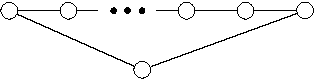
\includegraphics{A_series_ext_diag.pdf} & 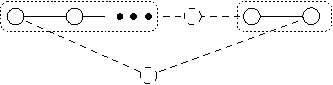
\includegraphics{A_series_ext_split.pdf} \\
  \hline
  $B_n$ & 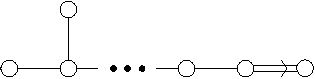
\includegraphics{B_series_ext_diag.pdf} & 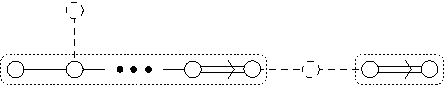
\includegraphics{B_series_ext_split.pdf} \\
  \hline
  $C_n$ & 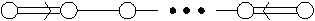
\includegraphics{C_series_ext_diag.pdf} & 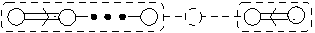
\includegraphics{C_series_ext_split.pdf} \\
  \hline
  $D_n$ & 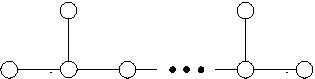
\includegraphics{D_series_ext_diag.pdf} & 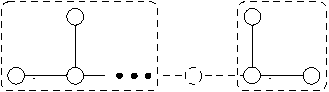
\includegraphics{D_series_ext_split.pdf} \\
  \hline
\end{tabular}
\caption{Subalgebras $\mathfrak{a},\; \mathfrak{a}_{\bot}$ for the classical series}}
\end{table}

For the algebra $\mathfrak{g}$ from the series $A_r$ the roots in the orthogonal basis $\{e_i,\; 1\leq i\leq r+1\}$ are $\Delta=\{\alpha_{ i j}= e_i- e_j,\; 1\leq i, j\leq r+1\}$, $\Delta^{+}=\{\alpha_{ij},\; i<j\}$ and the set of simple roots consists of $\alpha_{1,2},\alpha_{2,3},\dots,\alpha_{r,r+1}$. So for the regular subalgebra $\mathfrak{a}=A_{r_{\mathfrak{a}}}$ and its simple root system consisting of first $r_{\mathfrak{a}}$ simple roots we get $\Delta_{\mathfrak{a}_{\bot}}=\{\alpha_{ i j},\; r_{\mathfrak{a}}+1<i,j\leq r+1\}$ and $\mathfrak{a}_{\bot}=A_{r-r_{\mathfrak{a}}-1}$.

For the algebra $\mathfrak{g}$ from the series $B_r$ the roots in the orthogonal basis $\{e_i,\; 1\leq i\leq r\}$ are $\Delta=\{\alpha_{\pm i,\pm j}=\pm e_i\pm e_j,\;i<j;\; \alpha_{\pm j}=\pm e_{ j},\; 1\leq j\leq r\}$, $\Delta^{+}=\{\alpha_{i,-j},\; \alpha_{ij},\; \alpha_j;\; i<j,\; 1\leq j\leq r\}$ and the set of simple roots consists of $\alpha_{1,-2},\alpha_{2,-3},\dots,\alpha_{r-1,-r},\alpha_r$. So if the regular subalgebra $\mathfrak{a}=A_{r_{\mathfrak{a}}}$ and its simple root system consists of first $r_{\mathfrak{a}}$ simple roots, then $\Delta_{\mathfrak{a}_{\bot}}=\{\alpha_{\pm i,\pm j},\;\alpha_j,\; r_{\mathfrak{a}}+1<i<j\leq r\}$ and $\mathfrak{a}_{\bot}=B_{r-r_{\mathfrak{a}}-1}$. Otherwise if $\mathfrak{a}=B_{r_{\mathfrak{a}}}$ and its simple roots are $\alpha_{r-r_{\mathfrak{a}}+1,-r+r_{\mathfrak{a}}-2},\dots,\alpha_{r-1,r},\alpha_r$ we see that $\Delta_{\mathfrak{a}_{\bot}}=\{\alpha_{\pm i,\pm j},\;\alpha_j,\; 1<i<j\leq r-r_{\mathfrak{a}}\}$ and $\mathfrak{a}_{\bot}=B_{r-r_{\mathfrak{a}}}$. It is the only case when simple roots of $\mathfrak{a}_{\bot}$ can not be obtained from the extended Dynkin diagram, as can be seen in the Table \ref{tab:diagrams}.

For the algebra $\mathfrak{g}$ from the series $C_r$ the roots in the orthogonal basis $\{e_i,\; 1\leq i\leq r\}$ are $\Delta=\{\alpha_{\pm i,\pm j}=\pm e_i\pm e_j,\;i<j;\; \alpha_{\pm j}=\pm 2e_{ j},\; 1\leq j\leq r\}$, $\Delta^{+}=\{\alpha_{i,-j},\; \alpha_{ij},\; \alpha_j;\; i<j,\; 1\leq j\leq r\}$ and the set of simple roots consists of $\alpha_{1,-2},\alpha_{2,-3},\dots,\alpha_{r-1,-r},\alpha_r$. So if the regular subalgebra $\mathfrak{a}=A_{r_{\mathfrak{a}}}$ and its simple root system consists of first $r_{\mathfrak{a}}$ simple roots, then $\Delta_{\mathfrak{a}_{\bot}}=\{\alpha_{\pm i,\pm j},\;\alpha_j,\; r_{\mathfrak{a}}+1<i<j\leq r\}$ and $\mathfrak{a}_{\bot}=C_{r-r_{\mathfrak{a}}-1}$. Otherwise if $\mathfrak{a}=C_{r_{\mathfrak{a}}}$ and its simple roots are $\alpha_{r-r_{\mathfrak{a}}+1,-r+r_{\mathfrak{a}}-2},\dots,\alpha_{r-1,r},\alpha_r$ we see that $\Delta_{\mathfrak{a}_{\bot}}=\{\alpha_{\pm i,\pm j},\;\alpha_j,\; 1<i<j\leq r-r_{\mathfrak{a}}\}$ and $\mathfrak{a}_{\bot}=C_{r-r_{\mathfrak{a}}}$.

For the algebra $\mathfrak{g}$ from the series $D_r$ the roots in the orthogonal basis $\{e_i,\; 1\leq i\leq r\}$ are $\Delta=\{\alpha_{\pm i,\pm j}=\pm e_i\pm e_j,\;1\leq i<j\leq r\}$, $\Delta^{+}=\{\alpha_{i,-j},\; \alpha_{ij},\; i<j,\; 1\leq j\leq r\}$ and the set of simple roots consists of $\alpha_{1,-2},\alpha_{2,-3},\dots,\alpha_{r-1,-r},\alpha_{r-1,r}$. So if the regular subalgebra $\mathfrak{a}=A_{r_{\mathfrak{a}}}$ and its simple root system consists of first $r_{\mathfrak{a}}$ simple roots, then $\Delta_{\mathfrak{a}_{\bot}}=\{\alpha_{\pm i,\pm j},\; r_{\mathfrak{a}}+1<i<j\leq r\}$ and $\mathfrak{a}_{\bot}=D_{r-r_{\mathfrak{a}}-1}$. Otherwise if $\mathfrak{a}=D_{r_{\mathfrak{a}}}$ and its simple roots are $\alpha_{r-r_{\mathfrak{a}}+1,-r+r_{\mathfrak{a}}-2},\dots,\alpha_{r-1,r},\alpha_{r-1,r}$ we see that $\Delta_{\mathfrak{a}_{\bot}}=\{\alpha_{\pm i,\pm j},\; 1<i<j\leq r-r_{\mathfrak{a}}\}$ and $\mathfrak{a}_{\bot}=D_{r-r_{\mathfrak{a}}}$.

(In the case of special embeddings the set $\Delta^{+}_{\bot}$ can be empty as for the
special embedding of $A_1\subset A_2$ with the embedding index equal to 4, or non-empty for example for the embedding $A_1\subset A_2\subset A_3$ which is depicted at the Figure \ref{fig:a1a2a3}. {\color{red}(This is for us!)})
\begin{figure}[ph]
\noindent  \centering{
  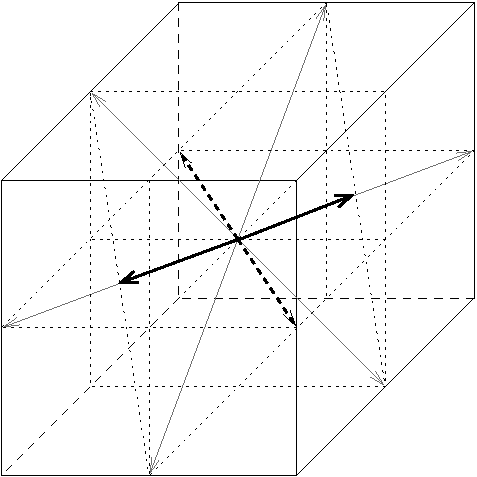
\includegraphics[width=120mm]{special_A1_A2_A3.pdf}
  \caption{Special embedding $A_1\subset A_2\subset A_3$. Grey vectors are the roots of $A_2$, thick black - of $\mathfrak{a}=A_1$, dashed black are the orthogonal roots of $A_1$ which is contained in $\mathfrak{a}_{\bot}$ }
}
  \label{fig:a1a2a3}
\end{figure}

Using the existing classification of maximal special subalgebras \cite{dynkin1952semisimple} we immediately have the following pairs of the orthogonal subalgebras $\mathfrak{a},\;\mathfrak{a}_{\bot}$
\begin{equation}
  \label{eq:42}
  \begin{array}{lll}
      su(p)\oplus su(q) & \subset su(pq) &\\
      so(p)\oplus so(q) & \subset so(pq) &\\
      sp(2p)\oplus sp(2q) & \subset so(4pq)&\\
      sp(2p)\oplus so(q) & \subset sp(2pq)&\\
      so(p)\oplus so(q) & \subset so(p+q)& \text{for}\;p\;\text{and}\;q\;\text{odd}\\
  \end{array}
\end{equation}
{\color{blue} Exceptional Lie algebras and other non-maximal subalgebras will be considered elsewhere.}

{\color{blue} Up to this point we considered the problem of $\mathfrak{a}_{\bot}$-construction given $\mathfrak{a}\in\mathfrak{g}$ for regular injections in terms of Dynkin diagrams. When the root systems $ \Delta$ and $\Delta_{\mathfrak{a}}$ are known explicitly all that we need is to select the roots  
$\Delta_{\bot}=\left\{\alpha\in \Delta:\alpha\bot \Delta_{\mathfrak{a}}\right\}$ and correspondingly the positive roots
$\Delta^{+}_{\bot}=\left\{\alpha\in \Delta^{+}:\alpha\bot \Delta_{\mathfrak{a}}\right\}$. }

Now consider the $\mathfrak{a}_{\bot}\oplus\mathfrak{h}$-module 
{\color{red} What is $\mathfrak{h}$? If it is the Cartan of $\mathfrak{g}$ then there are too many Cartans! It must be $\mathfrak{h}_{\mathfrak{a}}$.}
with the highest weight $\mu$. For the character of this module we have
\begin{equation}
  \label{eq:41}
  ch L^{\mu}_{\mathfrak{a}_{\bot}\oplus \mathfrak{h}}= \frac{\sum_{\omega\in W_{\bot}} \epsilon(\omega) e^{\omega(\mu+\rho_{\mathfrak{a}_{\bot}})-\rho_{\mathfrak{a}_{\bot}}}}{\prod_{\alpha\in\Delta^{+}_{\bot}}(1-e^{-\alpha})^{\mathrm{mult}(\alpha)}}
\end{equation}
The projection $\pi_{\mathfrak{a}}(ch\, L^{\mu}_{\mathfrak{a}_{\bot}\oplus \mathfrak{h}})$ gives us the single element $e^{\pi_{\mathfrak{a}} \cdot\mu}$ of the formal algebra ${\cal E}\left( \mathfrak{a}\right)$ with the multiplicity equal to the dimension of the module $L^{\mu}_{\mathfrak{a}_{\bot}\oplus \mathfrak{h}}$, since all the roots of $\mathfrak{a}_{\bot}$ are orthogonal to  that of $\Delta_{\mathfrak{a}}$.

Using this property we can reconsider the restriction $ch\, L^{\mu}_{\mathfrak{g}\downarrow \mathfrak{a}_{\bot}\oplus \mathfrak{h}}$, that is the character of the direct sum of $\mathfrak{a}_{\bot}\oplus\mathfrak{h}$-modules.
Multiply the equation (\ref{eq:4}) by the element
\begin{equation}
  \label{eq:5}
  \pi_{\mathfrak{a}}\left(\prod_{\alpha\in \Delta^{+}\setminus \Delta^{+}_{\bot}}(1-e^{-\alpha})^{\mathrm{mult}_{\mathfrak{g}}(\alpha)} \right)
\end{equation}
{\color{red}(This term is non-zero.) --This is for us.}
{\color{blue}Taking into account that for any formal series $Q \in {\cal E}$ and the binomial the projection commutes with the multiplication,
\begin{equation}
  \label{eq:6}
  \pi_{\mathfrak{a}} (Q) \pi_{\mathfrak{a}}(1-e^{-\alpha})=\pi_{\mathfrak{a}}\left(Q\cdot (1-e^{-\alpha})\right),
\end{equation}
we can rewrite the 
product of (\ref{eq:4}) and (\ref{eq:5}) in the form:}
\begin{multline}
  \label{eq:7}
  \pi_{\mathfrak{a}}\left(\frac{\sum_{\omega\in W} \epsilon(\omega) e^{\omega(\mu+\rho)-\rho}}{\prod_{\alpha\in\Delta^{+}_{\bot}}(1-e^{-\alpha})^{\mathrm{mult}(\alpha)}}\right) = \\
  \pi_{\mathfrak{a}}\left(\prod_{\alpha\in \Delta^{+}\setminus \Delta^{+}_{\bot}}(1-e^{-\alpha})^{\mathrm{mult}_{\mathfrak{g}}(\alpha)} \right)\sum_{\nu\in P^{+}_{\mathfrak{a}}}b^{(\mu)}_{\nu}
  \frac{\sum_{\omega\in W_{\mathfrak{a}}}\epsilon(\omega)e^{\omega(\nu+\rho_{\mathfrak{a}})-\rho_{\mathfrak{a}}}}{\prod_{\beta\in \Delta_{\mathfrak{a}}^{+}}(1-e^{-\beta})^{\mathrm{mult}_{\mathfrak{a}}(\beta)}}
\end{multline}
The right-hand side of this equation can be reorganised similarly to what was performed in the paper \cite{ilyin812pbc}, by introducing the anomalous branching coefficients $k_{\lambda}$,
\begin{equation}
  \label{eq:10}
  \sum_{\nu \in P_{\frak{a}}}b_{\nu }^{\left( \mu \right) }\Psi _{\left( \frak{%
        a}\right) }^{\left( \nu \right) }=\sum_{\lambda \in P_{\frak{a}}}k_{\lambda
  }^{\left( \mu \right) }e^{\lambda }
\end{equation}
and simplifying the multiplier:
\begin{multline}
  \label{eq:12}
  \pi_{\mathfrak{a}}\left(\frac{\sum_{\omega\in W} \epsilon(\omega) e^{\omega(\mu+\rho)-\rho}}{\prod_{\alpha\in\Delta^{+}_{\bot}}(1-e^{-\alpha})^{\mathrm{mult}(\alpha)}}\right) = \\
  \left(\prod_{\alpha\in \pi_{\mathfrak{a}}\left(\Delta^{+}\setminus \Delta^{+}_{\bot}\right)}(1-e^{-\alpha})^{{\rm mult}_{\mathfrak{g}}(\alpha)-{\rm mult}_{\mathfrak{a}}(\alpha)} \right)
    \sum_{\lambda \in P_{\frak{a}}}k_{\lambda}^{\left( \mu \right) }e^{\lambda }
\end{multline}


If the set $\Delta^{+}_{\bot}$ is non-empty then the Weyl reflections corresponding to the positive roots of $\Delta^{+}_{\bot}$ generate a subgroup $W_{\bot}$ of the Weyl group $W$.
{\color{red} (We have denoted the subalgebra with the root space spanned over the set $\Delta^{+}_{\bot}$ by $\mathfrak{a}_{\bot}$) we are well acquainted with this!}
Let us reorganise the summation in the left-hand side of (\ref{eq:12}).
Consider the factor-space $W_{\bot}\backslash W$. For the class $\tilde{\omega}\in W_{\bot}\backslash W$ choose the representative $\omega \in \tilde{\omega}$ such that 
{\color{red} $\omega(\mu+\rho)\in \bar{C}_{\mathfrak{a}_{\bot}}$. This is a mistake. Such a transformation may not exist. We can only insist on } $\pi_{\mathfrak{a}_{\bot}}\omega(\mu+\rho)\in \bar{C}_{\mathfrak{a}_{\bot}}$,
\begin{multline}
  \label{eq:13}
 \pi_{\mathfrak{a}}\left(\frac{\sum_{\omega\in W} \epsilon(\omega) e^{\omega(\mu+\rho)-\rho}}{\prod_{\alpha\in\Delta^{+}_{\bot}}(1-e^{-\alpha})^{\mathrm{mult}(\alpha)}}\right) = \\
 \pi_{\mathfrak{a}}\left(\sum_{\omega\in W_{\bot}\backslash W} \epsilon(\omega) \frac{\sum_{\nu\in W_{\bot}}\epsilon(\nu) e^{\nu \cdot \omega(\mu+\rho)-\rho}}{\prod_{\alpha\in\Delta^{+}_{\bot}}(1-e^{-\alpha})^{\mathrm{mult}(\alpha)}}\right)
\end{multline}
The fraction in the right-hand side of the equation is similar to the character of some  $\mathfrak{a}_{\bot}$-module.
Let us rewrite the shifted weights
\begin{equation}
  \label{eq:30}
  \nu\cdot\omega(\mu+\rho)-\rho=\nu\cdot \bigl(\omega(\mu+\rho)-\pi_{\mathfrak{a}}(\omega(\mu+\rho))-\rho_{\mathfrak{a}_{\bot}}+\rho_{\mathfrak{a}_{\bot}}+\pi_{\mathfrak{a}}(\omega(\mu+\rho))\bigr)-\rho
\end{equation}

Since $\nu\cdot \pi_{\mathfrak{a}}(\omega(\mu+\rho))=\pi_{\mathfrak{a}}(\omega(\mu+\rho))$ and $\omega(\mu+\rho)-\pi_{\mathfrak{a}}(\omega(\mu+\rho))=\pi_{\mathfrak{a}_{\bot}}(\omega(\mu+\rho))$, we get
\begin{multline}
  \label{eq:14}
  \sum_{\omega\in W_{\bot}\backslash W} \epsilon(\omega) \frac{\sum_{\nu\in W_{\bot}}\epsilon(\nu) e^{\nu \cdot \omega(\mu+\rho)-\rho}}{\prod_{\alpha\in\Delta^{+}_{\bot}}(1-e^{-\alpha})^{\mathrm{mult}(\alpha)}} =\\
  \sum_{\omega\in W_{\bot}\backslash W} \epsilon(\omega) e^{\pi_{\mathfrak{a}}(\omega(\mu+\rho))-\rho} \frac{e^{\rho_{\mathfrak{a}_{\bot}} }\sum_{\nu\in W_{\bot}}\epsilon(\nu) e^{\nu \cdot (\pi_{\mathfrak{a}_{\bot}}(\omega(\mu+\rho))-\rho_{\mathfrak{a}_{\bot}}+\rho_{\mathfrak{a}_{\bot}})-\rho_{\mathfrak{a}_{\bot}}}}{\prod_{\alpha\in\Delta^{+}_{\bot}}(1-e^{-\alpha})^{\mathrm{mult}(\alpha)}}=\\
  \sum_{\omega\in W_{\bot}\backslash W} \epsilon(\omega) e^{\pi_{\mathfrak{a}}(\omega(\mu+\rho))-\rho}e^{\rho_{\mathfrak{a}_{\bot}}} {\rm ch} L^{\pi_{\mathfrak{a}_{\bot}}(\omega(\mu+\rho))-\rho_{\mathfrak{a}_{\bot}}}_{\mathfrak{a}_{\bot}}
\end{multline}
The projector $\pi_{\mathfrak{a}}$ transforms the character of the module ${\rm ch}L^{\pi_{\mathfrak{a}_{\bot}}(\omega(\mu+\rho))-\rho_{\mathfrak{a}_{\bot}}}_{\mathfrak{a}_{\bot}}$ into an element equal to the dimension of the module multiplied by the unit element {\color{red}" of the algebra of formal exponents" (for us)}:
  \begin{multline}
    \label{eq:15}
    \pi_{\mathfrak{a}}\left( \sum_{\omega\in W_{\bot}\backslash W} \epsilon(\omega) e^{\pi_{\mathfrak{a}}(\omega(\mu+\rho))-\rho}e^{\rho_{\mathfrak{a}_{\bot}}} \mathrm{ch} L^{\pi_{\mathfrak{a}_{\bot}}(\omega(\mu+\rho))-\rho_{\mathfrak{a}_{\bot}}}_{\mathfrak{a}_{\bot}}\right) = \\
    \sum_{\omega\in W_{\bot}\backslash W} \epsilon(\omega)\; \mathrm{dim}\left(L^{\pi_{\mathfrak{a}_{\bot}}(\omega(\mu+\rho))-\rho_{\mathfrak{a}_{\bot}}}_{\mathfrak{a}_{\bot}}\right) e^{\pi_{\mathfrak{a}}(\omega(\mu+\rho)-\rho)}
  \end{multline}
{\color{red} These dimensions of the modules could be easily calculated using the Weyl formula. (for us)}

Thus we have the equality
\begin{multline}
  \label{eq:9}
  \sum_{\omega\in W_{\bot}\backslash W} \epsilon(\omega) \mathrm{dim}\left(L^{\pi_{\mathfrak{a}_{\bot}}(\omega(\mu+\rho))-\rho_{\mathfrak{a}_{\bot}}}_{\mathfrak{a}_{\bot}}\right) e^{\pi_{\mathfrak{a}}(\omega(\mu+\rho)-\rho)}=\\
  \left(\prod_{\alpha\in \pi_{\mathfrak{a}}\left(\Delta^{+}\setminus \Delta^{+}_{\bot}\right)}(1-e^{-\alpha})^{{\rm mult}_{\mathfrak{g}}(\alpha)-{\rm mult}_{\mathfrak{\alpha}}} \right)
  \sum_{\lambda \in P_{\frak{a}}}k_{\lambda}^{\left( \mu \right) }e^{\lambda }
\end{multline}
Following the transformations performed in \cite{ilyin812pbc} we rewrite the multiplier in the right-hand side:
\begin{equation}
  \label{eq:11}
    \prod_{\alpha\in \pi_{\mathfrak{a}}\circ (\Delta^{+}\setminus \Delta^{+}_{\bot})} \left(1-e^{-\alpha}\right)^{\mathrm{mult}(\alpha)-\mathrm{mult}_{\mathfrak{a}}(\alpha)}=
     -\sum_{\gamma\in P_{\mathfrak{a}}} s(\gamma)e^{-\gamma}
\end{equation}

For the coefficient function $s\left( \gamma \right) $ define the carrier $\Phi _{\frak{a%
}\subset \frak{g}}\subset P_{\frak{a}}$:
\begin{equation}
\Phi _{\frak{a}\subset \frak{g}}=\left\{ \gamma \in P_{\frak{a}}\mid s\left(
\gamma \right) \neq 0\right\} ;  \label{phi-d}
\end{equation}
In these terms the equation for the formal elements,
\begin{multline}
  \label{eq:16}
  \sum_{\omega\in W_{\bot}\backslash W} \epsilon(\omega) \mathrm{dim}\left(L^{\pi_{\mathfrak{a}_{\bot}}(\omega(\mu+\rho))-\rho_{\mathfrak{a}_{\bot}}}_{\mathfrak{a}_{\bot}}\right) e^{\pi_{\mathfrak{a}}(\omega(\mu+\rho)-\rho)}=\\
  = -\sum_{\gamma \in \Phi _{\frak{a}\subset \frak{g}}} s\left( \gamma \right) e^{-\gamma }\sum_{\lambda \in P_{\frak{a}}}
  k_{\lambda }^{\left( \mu \right) }e^{\lambda } \\
  =-\sum_{\gamma \in \Phi _{\frak{a}\subset \frak{g}}}\sum_{\lambda \in P_{\frak{a}}}s\left( \gamma \right) k_{\lambda }^{\left( \mu \right)}e^{\lambda -\gamma }
\end{multline}
leads to the following equality 
\begin{equation}
  \label{eq:17}
   \sum_{\omega\in W_{\bot}\backslash W} \epsilon(\omega) \mathrm{dim}\left(L^{\pi_{\mathfrak{a}_{\bot}}(\omega(\mu+\rho))-\rho_{\mathfrak{a}_{\bot}}}_{\mathfrak{a}_{\bot}}\right) \delta_{\xi,\pi_{\mathfrak{a}}(\omega(\mu+\rho)-\rho)}+
   \sum_{\gamma \in \Phi _{\frak{a}\subset \frak{g}}} s(\gamma)\; k^{(\mu)}_{\xi+\gamma}=0;\quad \xi\in P_{\mathfrak{a}}
\end{equation}

To get the recurrent relations for the anomalous branching coefficients we use the following procedure  (similar to that in \cite{ilyin812pbc}).
Let $\gamma_{0} $ be the lowest vector with respect to the natural ordering in $%
\overset{\circ }{\Delta _{\frak{a}}}$ in the lowest grade of $\Phi _{\frak{a}\subset \frak{g}}$ and decompose the defining relation (\ref{eq:11}),
\begin{equation}
  \label{eq:18}
  \prod_{\alpha\in \pi_{\mathfrak{a}}\circ (\Delta^{+}\setminus \Delta^{+}_{\bot})}\left(
    1-e^{-\alpha }\right) ^{\mathrm{{mult}\left( \alpha \right) -{mult}}_{\frak{a%
      }}\mathrm{\left( \alpha \right) }}=-s\left( \gamma _{0}\right) e^{-\gamma
    _{0}}-\sum_{\gamma \in \Phi _{\frak{a}\subset \frak{g}}\setminus \left\{\gamma_{0}\right\}}s\left( \gamma \right) e^{-\gamma },
\end{equation}
then the equality (\ref{eq:17}) leads to the desired recurrent  relation for the anomalous branching coefficients:
\begin{multline}
  k_{\xi }^{\left( \mu \right) }=
  -\frac{1}{s\left( \gamma _{0}\right) }
  \left(
    \sum_{\omega\in W_{\bot}\backslash W} \epsilon(\omega)\; \mathrm{dim}
    \left(L^{\pi_{\mathfrak{a}_{\bot}}(\omega(\mu+\rho))-\rho_{\mathfrak{a}_{\bot}}}_{\mathfrak{a}_{\bot}}\right)
    \delta_{\xi-\gamma_0,\pi_{\mathfrak{a}}(\omega(\mu+\rho)-\rho)}+
    \right.\\
    \left. +
    \sum_{\gamma \in \Gamma _{\frak{a}\subset \frak{g}}} s\left( \gamma +\gamma _{0}\right) k_{\xi+\gamma }^{\left( \mu \right) }
  \right)
\label{recurrent relation}
\end{multline}
where the set
\begin{equation}
\Gamma _{\frak{a}\subset \frak{g}}=\left\{ \xi -\gamma _{0}|\xi \in \Phi _{%
\frak{a}\subset \frak{g}}\right\} \setminus \left\{ 0\right\} 
\label{fan-defined}
\end{equation}
 was introduced that is called the injection fan.


{\color{red}(If the set $\Delta_{\bot}^{+}$ is empty the modules $L_{\mathfrak{a}_{\bot}}$ are trivial, the dimensions are equal to 1 and we get the following formula (11) \eqref{eq:40} from the paper \cite{ilyin812pbc}) This is not true! And the formula presented is not the one that was thus generalized.} 
{\color{blue} Now let the set $\Delta_{\bot}^{+}$ be empty. There are three different reasons for $\Delta_{\bot}^{+}=0$: i) $\mathrm{dim}\mathfrak{h}_{\mathfrak{a}}=\mathrm{dim}\mathfrak{h}_{\mathfrak{g}}$, ii) $\mathfrak{a}_{\bot}=0$ and iii) $\mathfrak{a}_{\bot}\subset \mathfrak{h}_{\mathfrak{g}}$. Both the first and the second cases can be treated as corresponding to the trivial orthogonal subalgebra: 
$\mathfrak{a}_{\bot}=0$. In any of these cases instead of the formal characters in the right-hand side of (\ref{eq:13}) we obtain the formal element $e^{ \pi_{\mathfrak{a}_{\bot}}\omega(\mu+\rho)}$
In the first two cases (equivalent to $\mathfrak{a}_{\bot}=0$) the projection operator retains its purely geometrical meaning: the vector $\omega(\mu+\rho)$ is projected to the subspace orthogonal to the weight space of $\mathfrak{a}$. It is clear that in any of the three variants the final vector $\pi_{\mathfrak{a}}\pi_{\mathfrak{a}_{\bot}}\omega(\mu+\rho)$ leads to the unit of the formal algebra 
$\mathcal{E}$. Thus when the set $\Delta_{\bot}^{+}$ is empty we get the more simple recurrent relation: 
\begin{equation}
k_{\xi }^{\left( \mu \right) }=-\frac{1}{s\left( \gamma _{0}\right) }\left(
\sum_{w\in W}\epsilon \left( w\right) \delta _{\xi ,\pi _{\frak{a}}\circ
\left( w\circ (\mu +\rho )-\rho \right) +\gamma _{0}}+\sum_{\gamma \in
\Gamma _{\frak{a}\subset \frak{g}}}s\left( \gamma +\gamma _{0}\right) k_{\xi
+\gamma }^{\left( \mu \right) }\right)   \label{recurrent relation special}
\end{equation}
It coinsides with the one obtained in \cite{ilyin812pbc} (formula (16)). }

  In the next section we describe an algorithm for the computation of branching coefficients based on the relation \eqref{recurrent relation}.

\subsection{Algorithm for the recursive computation of the branching coefficients}
\label{sec:algorithm}

We use the recurrent relation \eqref{recurrent relation} to formulate an algorithm for recursive computation of the branching coefficients. It is important to mention that the computation of the branching coefficients is performed without the  explicit construction of the module $L^{(\mu)}_{\mathfrak{g}}$ and any of the modules $L^{(\nu)}_{\mathfrak{a}}$.

The algorithm contains the following steps.
\begin{enumerate}
\item Construct the sets $\Delta^{+}$ and $\Delta_{\mathfrak{a}}^{+}$ of positive roots for the algebras $\mathfrak{a} \subset \mathfrak{g}$.
\item Select the positive roots $\alpha\in \Delta^{+}$ which are orthogonal to the root subspace of $\mathfrak{a}$ and form the set $\Delta^{+}_{\bot}$.
\item Construct the set $\widehat{\Psi^{(\mu)}}=\left\{\omega(\mu+\rho)-\rho;\; \omega\in W\right\}$ of the anomalous weights of the $\mathfrak{g}$-module $L^{(\mu)}$.
\item {\color{red}"Select those weights $\lambda=\omega(\mu+\rho)$ which lies in the closure of the main Weyl chamber of the algebra $\mathfrak{a}_{\bot}$."
 for  lies in the closure of the main Weyl chamber of the algebra $\mathfrak{a}_{\bot}$. The same mistake!} Select the weights $\left\{ \lambda=\omega(\mu+\rho) | \pi_{\mathfrak{a}_{\bot}}\lambda \in \bar{C}_{\mathfrak{a}_{\bot}} \right\}$ Since we have constructed the set $\Delta^{+}_{\bot}$ we can easily check wether the weight $\pi_{\mathfrak{a}_{\bot}}\lambda$ lies in the main Weyl chamber of $\mathfrak{a}_{\bot}$ by computing the scalar product of $\lambda$ with the roots of $\Delta^{+}_{\bot}$ that must be non-negative.
\item For $\lambda=\omega(\mu+\rho),\; \pi_{\mathfrak{a}_{\bot}}\lambda\in \bar{C}_{\mathfrak{a}_{\bot}}$ calculate the dimensions of the corresponding modules $\mathrm{dim}\left(L^{\pi_{\mathfrak{a}_{\bot}}(\omega(\mu+\rho))-\rho_{\mathfrak{a}_{\bot}}}_{\mathfrak{a}_{\bot}}\right)$ using the Weyl formula with the set $\Delta^{+}_{\bot}$.
\item Construct the set $\Gamma$ \eqref{fan-defined}.
\item Calculate the anomalous branching coefficients in the main Weyl
  chamber of the subalgebra $\mathfrak{a}$ using recurrent relation (\ref{recurrent relation}).
\end{enumerate}

If we are interested in the branching coefficients for the embedding of the finite-dimensional Lie algebra into the affine Lie algebra we can construct the set of the anomalous weights up to the required grade and use the steps 4-7 of the algorithm for each grade. We can also speed up the algorithm by one-time computation of the representatives of the conjugate classes $W_{\bot}\backslash W$.

The next section contains several examples computed using this algorithm.

\section{Examples}
\label{sec:examples}

\subsection{Finite dimensional Lie algebras}
\label{sec:finite-dimens-lie}

\subsubsection{Regular embedding of $A_1$ into $B_2$}
\label{sec:regul-embedd-a_1}

Consider the regular embedding of $A_1$ into $B_2$. Simple roots $\alpha_1, \alpha_2$ of $B_2$ are drawn as the thick vectors at the Figure \ref{fig:B2_A1}. We denote the corresponding Weyl reflections by $\omega_1, \omega_2$. Simple root $\beta$ of the embedded $A_1$ is equal to $\alpha_1+\alpha_2$.

Let's describe the reduction of fundamental representation of $B_2$ with the highest weight (in fundamental weight basis) equal to $(1,0)$.
\begin{figure}[ph]
  \noindent\centering{
    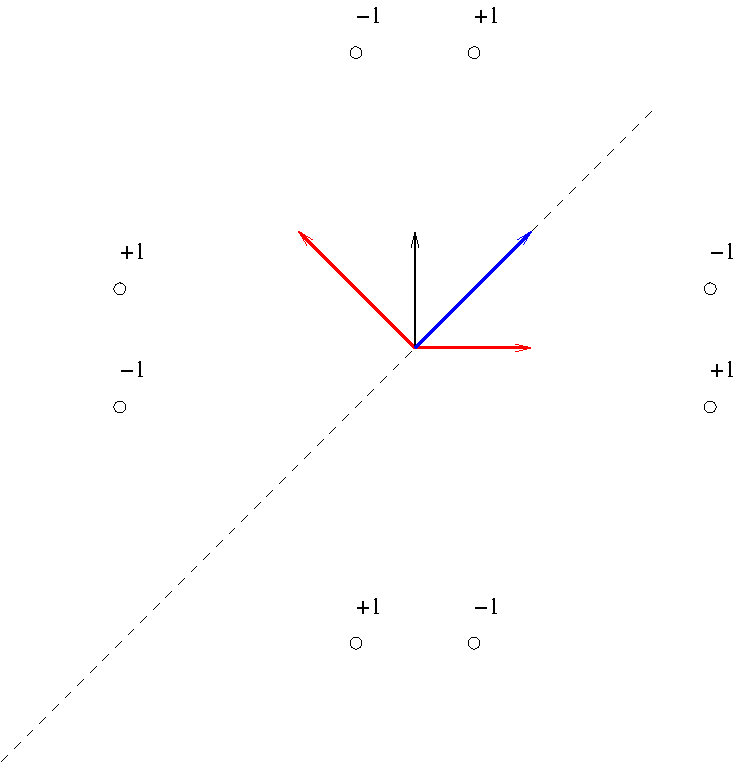
\includegraphics[width=90mm]{B2_A1.pdf}
  }
  \caption{Regular embedding of $A_1$ into $B_2$}
  \label{fig:B2_A1}
\end{figure}
On the Figure \ref{fig:B2_A1} we have also shown the set of points $\omega(\mu+\rho),\; \omega\in W$ of fundamental representation of $B_2$ with the corresponding determinants of Weyl reflections $\epsilon(\omega)$.
Now we have to factorise the Weyl group $W$ by $W_{\bot}=\left\{\omega_1\right\}$. We get the following set of anomalous points $\omega(\mu+\rho)-\rho,\; \omega\in W_{\bot}\backslash W$:
\begin{figure}[ph]
  \noindent\centering{
    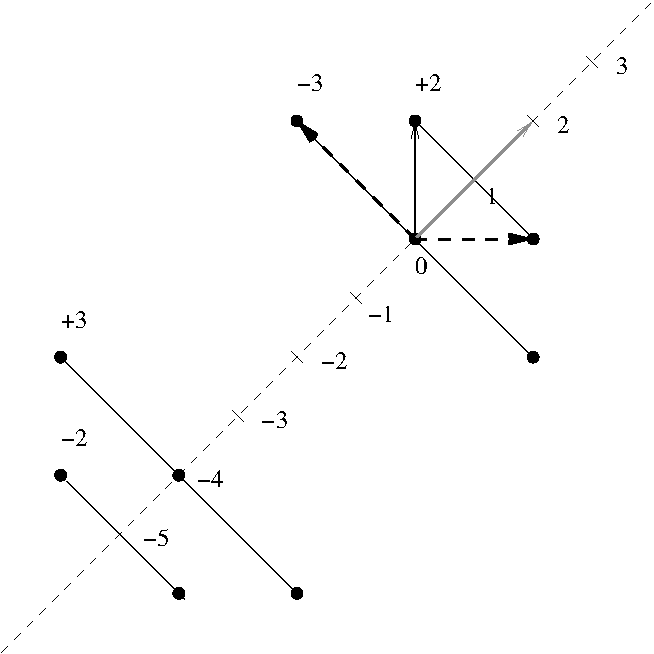
\includegraphics[width=90mm]{B2_A1_2.pdf}
  }
  \caption{Anomalous points and the corresponding $\mathfrak{a}_{\bot}=A_1$-modules}
  \label{fig:B2_A1_2}
\end{figure}
We have also depicted the corresponding $\mathfrak{a}_{\bot}=A_1$-modules $L^{\pi_{\mathfrak{a}_{\bot}}(\omega(\mu+\rho))-\rho_{\mathfrak{a}_{\bot}}}_{\mathfrak{a}_{\bot}}$.
Then we project these points and dimensions of modules onto the root space of subalgebra $\mathfrak{a}=A_1$ and get the following anomalous points in fundamental weights basis with corresponding multiplicities:
\begin{equation}
  \label{eq:25}
  (1,2),\; (0,-3),\; (-4,3),\; (-5,-2)
\end{equation}
For the function $s(\gamma)$ and the set $\Gamma$ from the definition (\ref{phi-d},\ref{fan-defined}) we have
\begin{equation}
  \label{eq:22}
  (1,2),\; (2,-1)
\end{equation}
Here the second component denotes the value of $s(\gamma)$.

Anomalous branching coefficient $k^{(1,0)}_{1}=2$, then for anomalous branching coefficient $k^{(1,0)}_{0}$ the formula (\ref{recurrent relation}) gives us
\begin{equation}
  \label{eq:23}
  k^{(1,0)}_{0}=-1\cdot k^{(1,0)}_2 +2\cdot k^{(1,0)}_1 - 3\cdot \delta_{0,0} = 1
\end{equation}
So we have computed the branching coefficients.

\subsubsection{Embedding of $B_2$ into $B_4$}
\label{sec:someth-high-dimens}
Consider the the regular embedding of the subalgebra $B_2$ into the algebra $B_4$.
We calculate the branching coefficients for the fundamental representation of $B_4$.
The corresponding Dynkin diagrams are in the Figure \ref{fig:dynkin}.
\begin{figure}[ph]
  \centering
  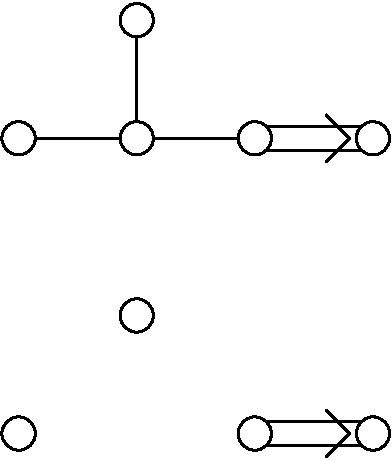
\includegraphics[width=60mm]{B4_B2_2A1.pdf}
  \caption{Dynkin diagrams}
  \label{fig:dynkin}
\end{figure}

In the orthogonal basis $e_1,\dots,e_4$ simple roots of $B_4$ are
\begin{equation}
  \label{eq:8}
  (e_1 - e_2,\; e_2 - e_3,\; e_3 - e_4,\; e_4)
\end{equation}
Positive roots are
\begin{multline}
  \label{eq:19}
  (e_1 - e_2,\; e_2 - e_3,\; e_3 - e_4,\; e_4,\; e_1 - e_3,\; e_2 - e_4,\; e_3 + e_4,\; e_3,\; e_1 - e_4,\;\\
    e_2 + e_4,\; e_2,\; e_1 + e_4,\; e_2 + e_3,\; e_1,\; e_1 + e_3,\; e_1 + e_2)
\end{multline}
Simple roots of the embedded subalgebra $\mathfrak{a}=B_2$ are
\begin{equation}
  \label{eq:26}
  (e_3-e_4,e_4)
\end{equation}

The set $\Delta^{+}_{\bot}$ is equal to
\begin{equation}
  \label{eq:27}
  \left\{e_1-e_2,e_1+e_2,e_1,e_2\right\}
\end{equation}

We see that this is the set of positive roots of the algebra $\mathfrak{a}_{\bot}=B_2$.

To find the branching coefficients we need to compute the anomalous points of $B_4$, select point lying in the main Weyl chamber of $\mathfrak{a}_{\bot}$ and compute the dimensions of corresponding $\mathfrak{a}_{\bot}$-modules.

We consider the $B_4$-module with the highest weight $\mu=(0,1,0,2)=2
e_1 + 2 e_2 + e_3 + e_4$.

The set of the anomalous points $\omega(\mu+\rho)-\rho,\; \omega\in W$
consists of 384 points. We do not show it here.

We need to select those points $\omega(\mu+\rho)$  which are projected into the main chamber of the embedded algebra $\mathfrak{a}_{\bot}$.
It means that scalar product of these points with all the roots from $\Delta^{+}_{\bot}$ is non-negative.

To compute dimensions of the corresponding
$\mathfrak{a}_{\bot}$-modules we need to project each selected point
onto the root space $\Delta^{+}_{\bot}$ and substract
$\rho_{\mathfrak{a}_{\bot}}$, then use Weyl dimension formula.

We show the result of this procedure on the Figure \ref{fig:B4B2anom}.
\begin{figure}[h!tb]
    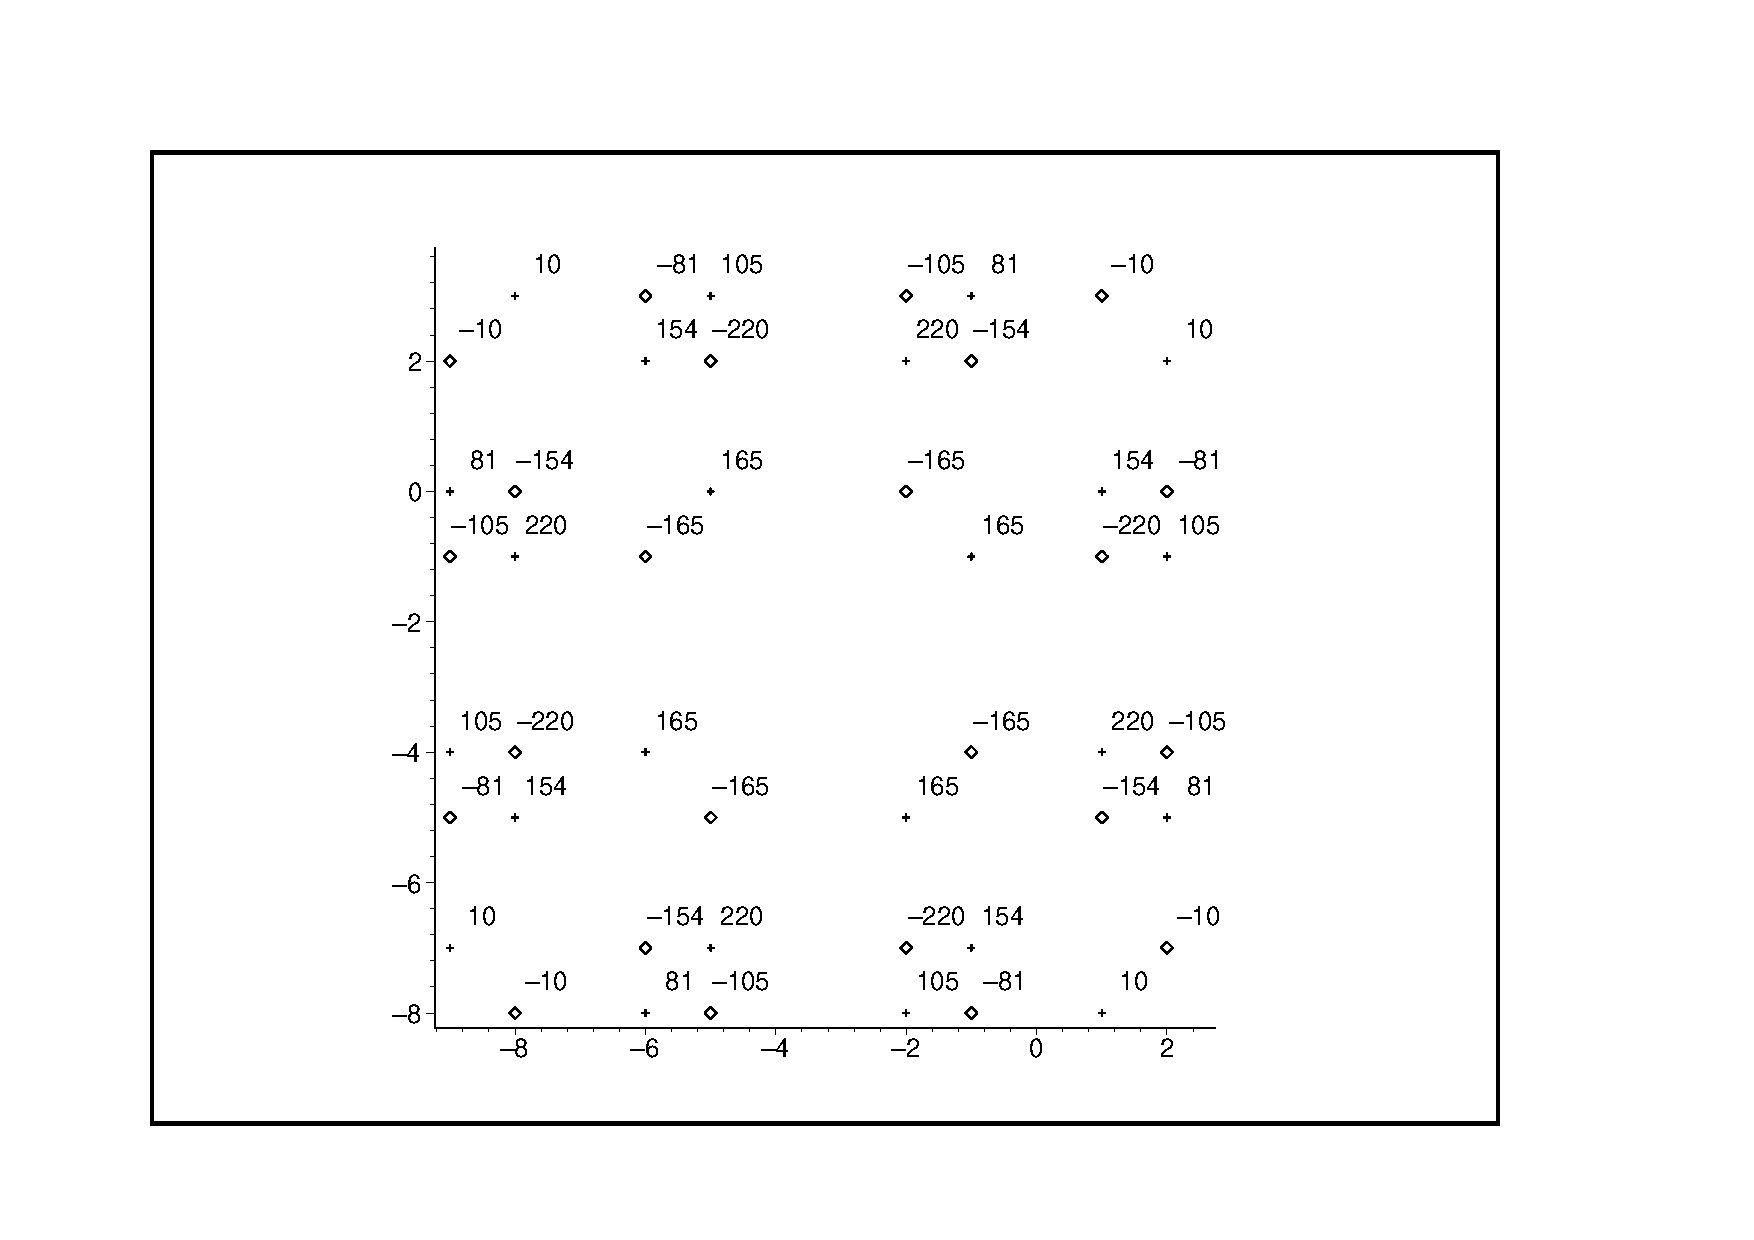
\includegraphics[width=130mm]{B4_B2_anom_points.pdf}
  \caption{Anomalous points with the dimensions of corresponding $\mathfrak{a}_{\bot}$-modules.}
  \label{fig:B4B2anom}
\end{figure}

Then we should construct ``the fan'' and use the recurrent relation for the computation of anomalous branching coefficients.

Using the definition (\ref{fan-defined}) we get the following set of
the points $\Gamma$ with the corresponding values $s(\gamma+\gamma_0)$, depicted at the Figure \ref{fig:B4B2Fan}.
\begin{figure}[h!tb]
  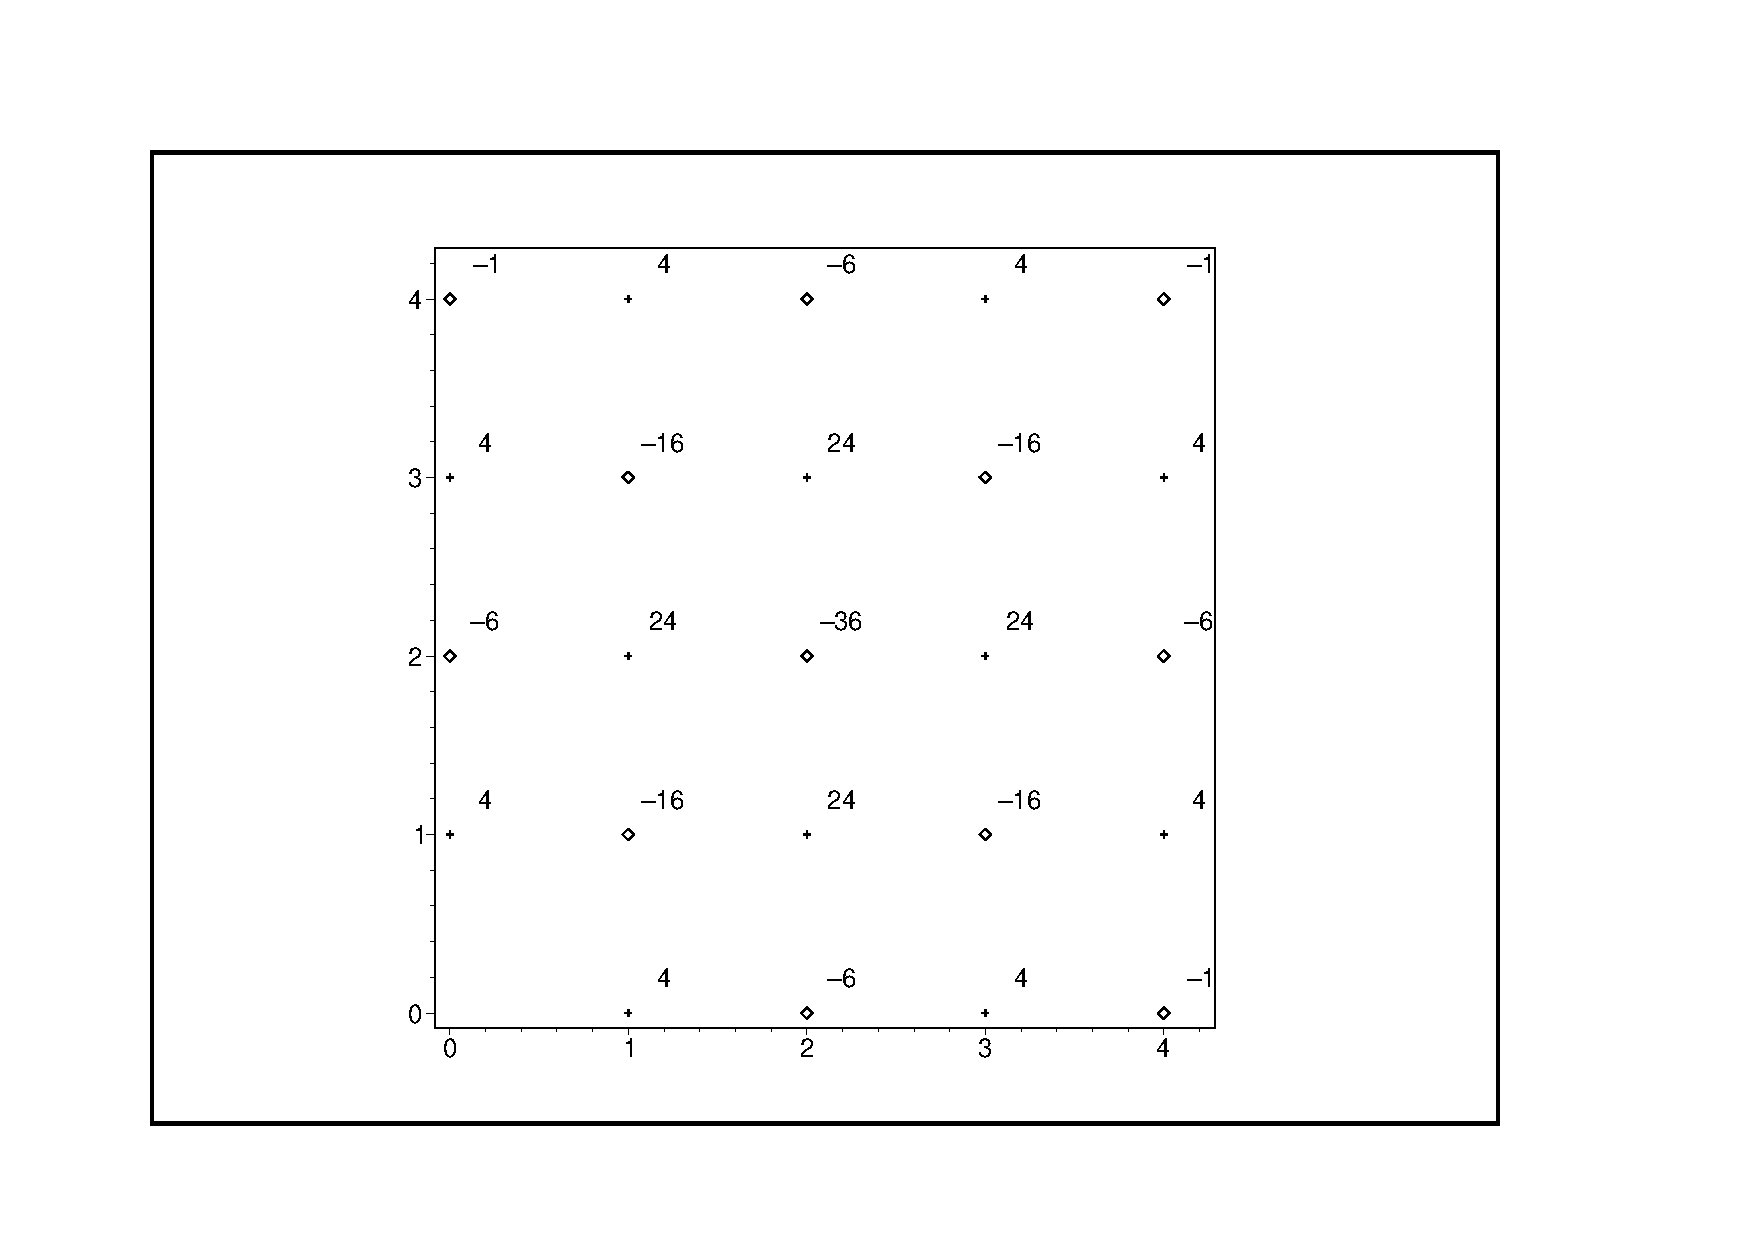
\includegraphics[width=130mm]{B4_B2_fan.pdf}
  \caption{Fan for $B_2\subset B_4$}
  \label{fig:B4B2Fan}
\end{figure}
We use the recurrent relation (\ref{recurrent relation}) and get
following branching coefficients:
\begin{equation}
  \label{eq:24}
  \pi_{\mathfrak{a}} \left(ch L^{(0,1,0,2)}_{B_4}\right) = 6 \; ch L^{(0,0)}_{B_2}+ 60
  \; ch L_{B_2}^{(0,2)}+ 30 \; ch L_{B_2}^{(1,0)}+ 19 \; ch L_{B_2}^{(2,0)}+
  40 \; ch L_{B_2}^{(1,2)}+ 10 \; ch L_{B_2}^{(2,2)}
\end{equation}
The dimension of the highest-weight $B_4$-module $L^{(0,1,0,2)}_{B_4}$
is equal to 2772. It is easy to see, that right-hand side of the
equation (\ref{eq:24}) gives the same result.


\subsection{Affine Lie algebras}
\label{sec:affine-lie-algebras}
\subsubsection{Embedding of the affine algebra into affine algebra}
\label{sec:embedd-affine-algebr}

Consider the affine extension of the example \ref{sec:regul-embedd-a_1}.
Since this embedding is regular, the level of the representations of the subalgebra is equal to the level of the representation of the algebra.

The set $\Delta^{+}_{\bot}$ of the orthogonal positive roots with the zero projection on the root space of the subalgebra $\hat{A_1}$ is the same as in the finite-dimensional case.

Consider the level one representation of the algebra $\mathfrak{g}=\hat{B_2}$ with the highest weight $w_1=(1,0,1,0)$, where the first two components are the coordinates of the classical part in the orthogonal basis $e_1,e_2$, the third is is the level of the weight and the fourth the grade.


The set of the anomalous points of this representation up to sixth grade is depicted in the Figure \ref{fig:affine_B2_anom_point} and in each grade it looks like in the Figure \ref{fig:B2_A1}.

\begin{figure}[h!tb]
  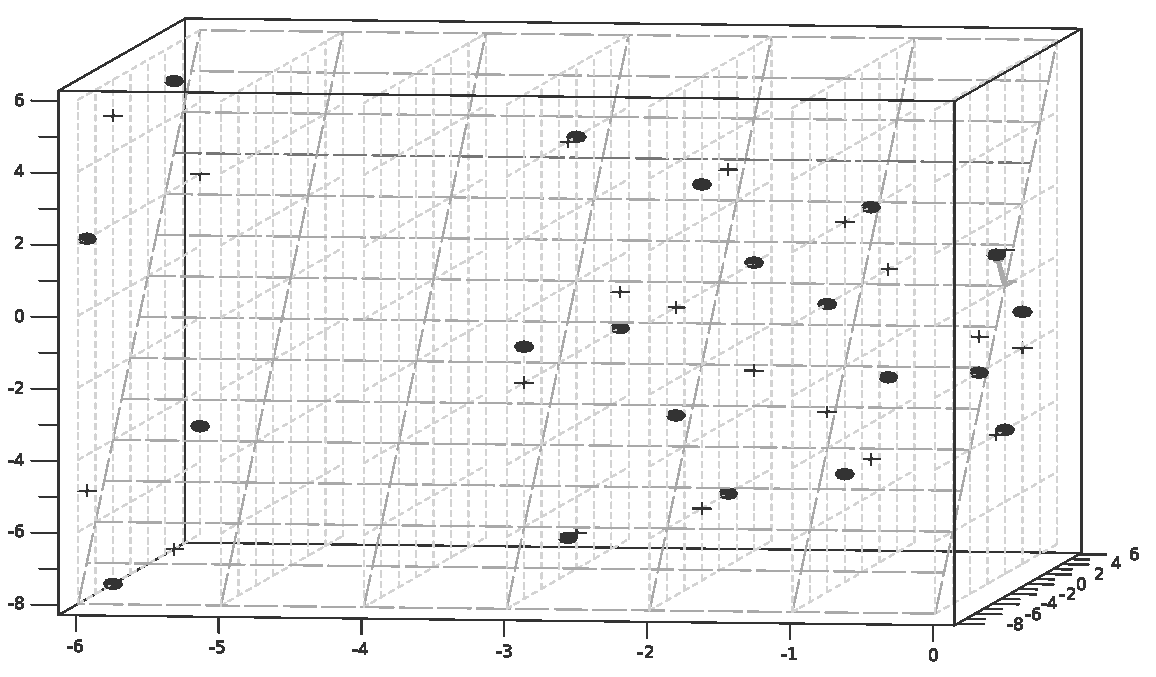
\includegraphics[width=160mm]{AffineB2_A1_Anom.pdf}
  \caption{The anomalous points of the $(1,0,1,0)$ representation of the algebra $\hat{B_2}$}
  \label{fig:affine_B2_anom_point}
\end{figure}

As the next step of our algorithm \ref{sec:algorithm} we project the anomalous points to the weight space of the subalgebra $\hat{A_1}$ and calculate the dimensions of the corresponding $\mathfrak{a}_{\bot}$-modules $L^{\pi_{\mathfrak{a}_{\bot}}(\omega(\mu+\rho))-\rho_{\mathfrak{a}_{\bot}}}_{\mathfrak{a}_{\bot}}$.
The result of this computation up to the twelfth grade is presented at the Figure
\begin{figure}[h!tb]
  \centering
  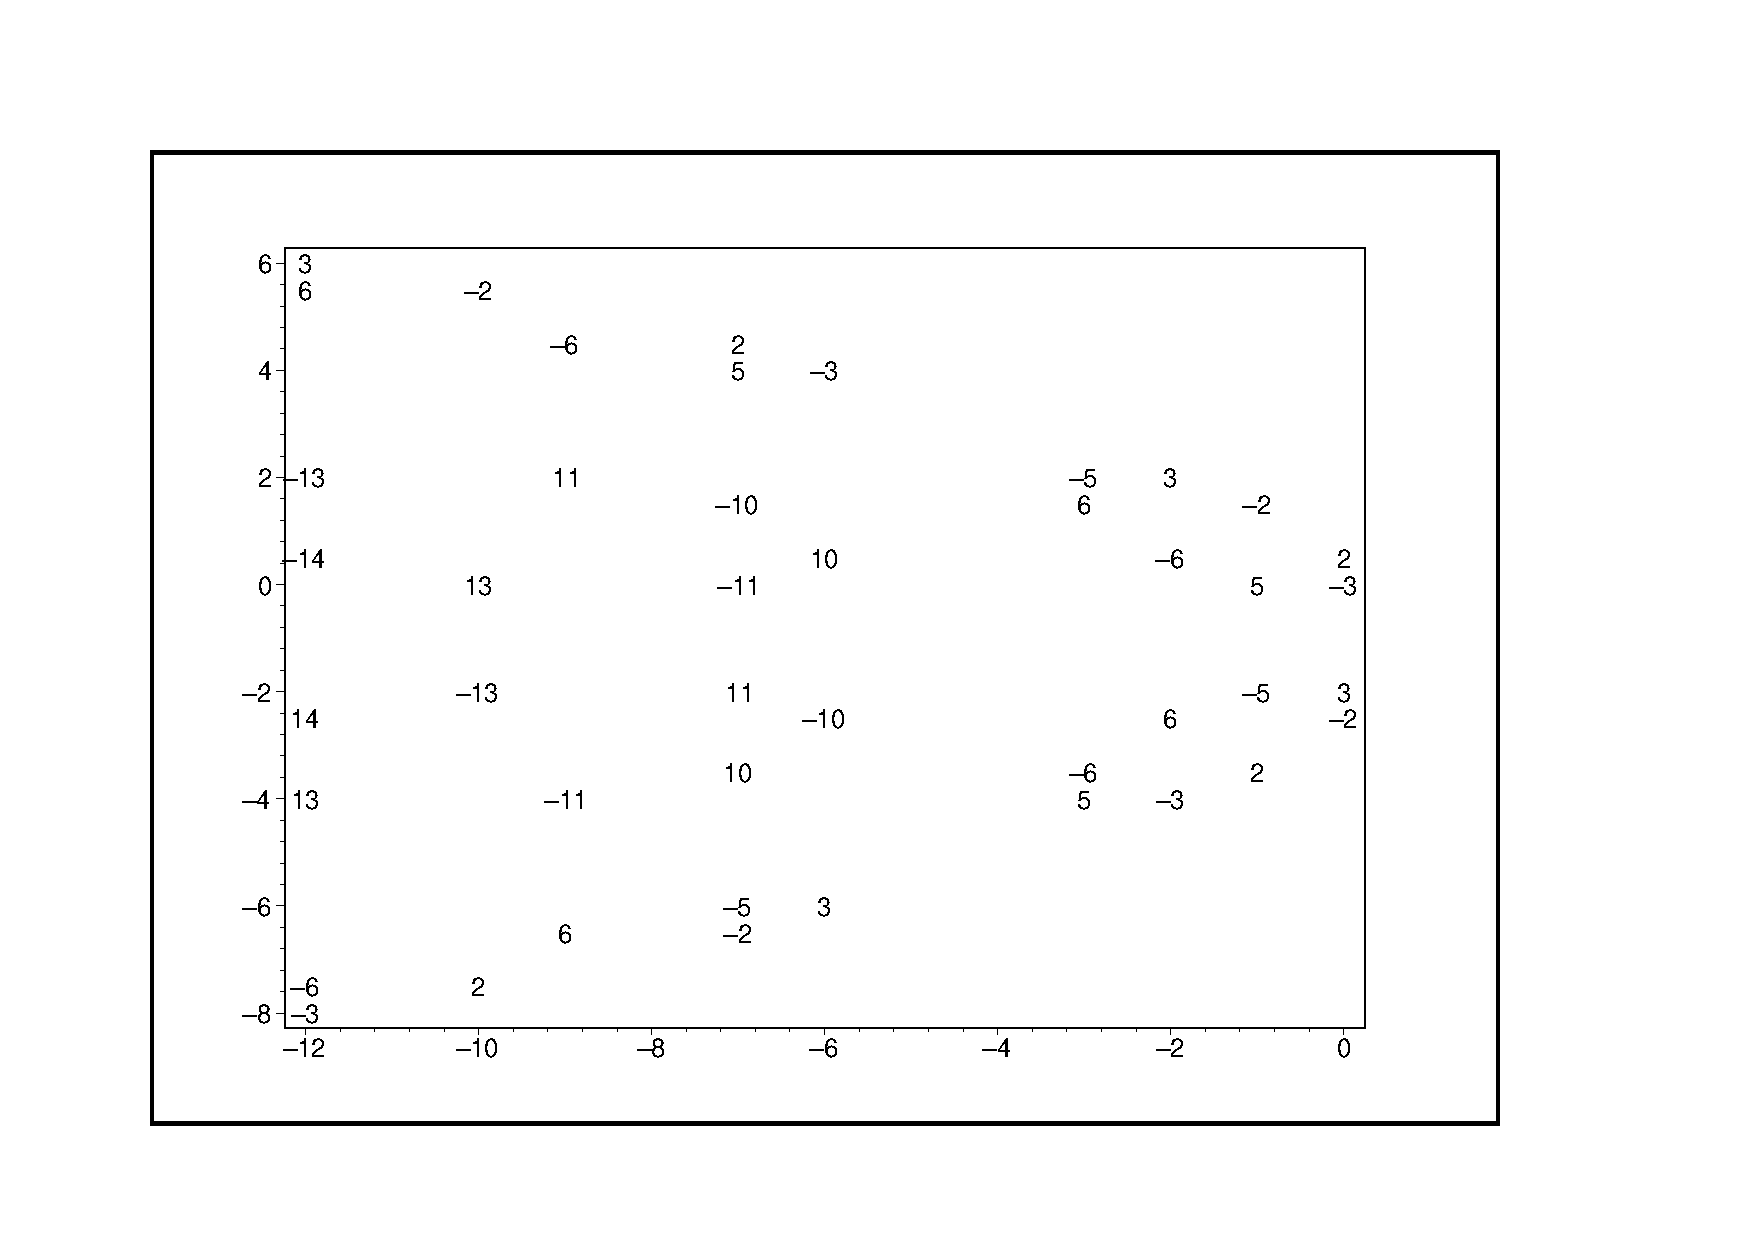
\includegraphics[width=150mm]{AffineB2_A1_proj_anom.pdf}
  \caption{Projected anomalous points and the dimensions of $\mathfrak{a}_{\bot}$-modules.}
  \label{fig:AffineB2_A1_anom_proj}
\end{figure}

Then we should construct ``the fan'' and use the recurrent relation for the computation of anomalous branching coefficients.

Using the definition (\ref{fan-defined}) we get the following set of
the points $\Gamma$ with the corresponding values $s(\gamma+\gamma_0)$: \ref{fig:AffineB2A1Fan}.
Here we restricted the computation to the twelfth grade.
\begin{figure}[ph]
  \centering
  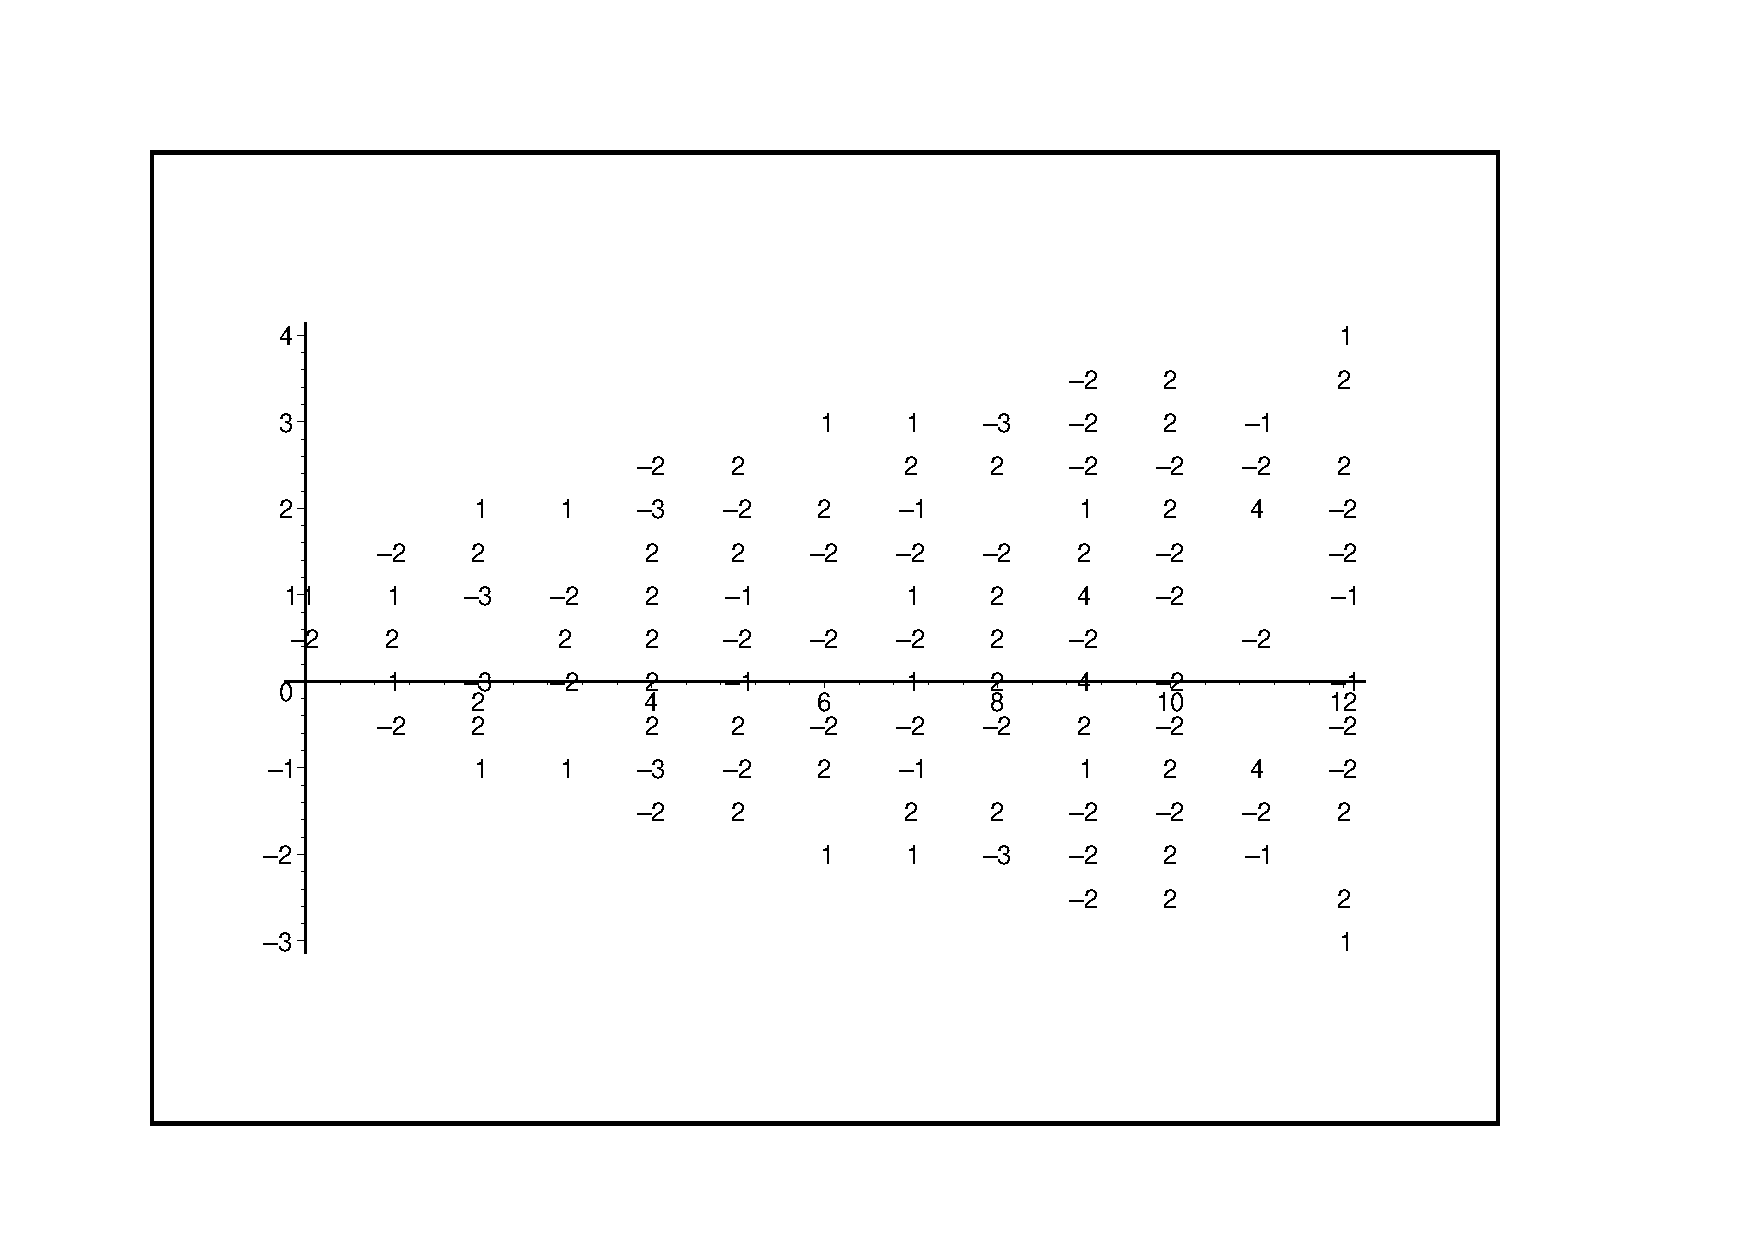
\includegraphics[width=130mm]{AffineB2_A1_fan.pdf}
  \caption{Fan for $\hat{A_1}\subset \hat{B_2}$}
  \label{fig:AffineB2A1Fan}
\end{figure}

Also we should mention that the lowest vector of the fan $\gamma_0$ is equal to zero, since we have excluded all the roots of $\Delta^{+}_{\bot}$ from the defining relation (\ref{fan-defined}).

Using the recurrent relation for the anomalous branching coefficients we get the following result
\begin{figure}[ph]
  \centering
  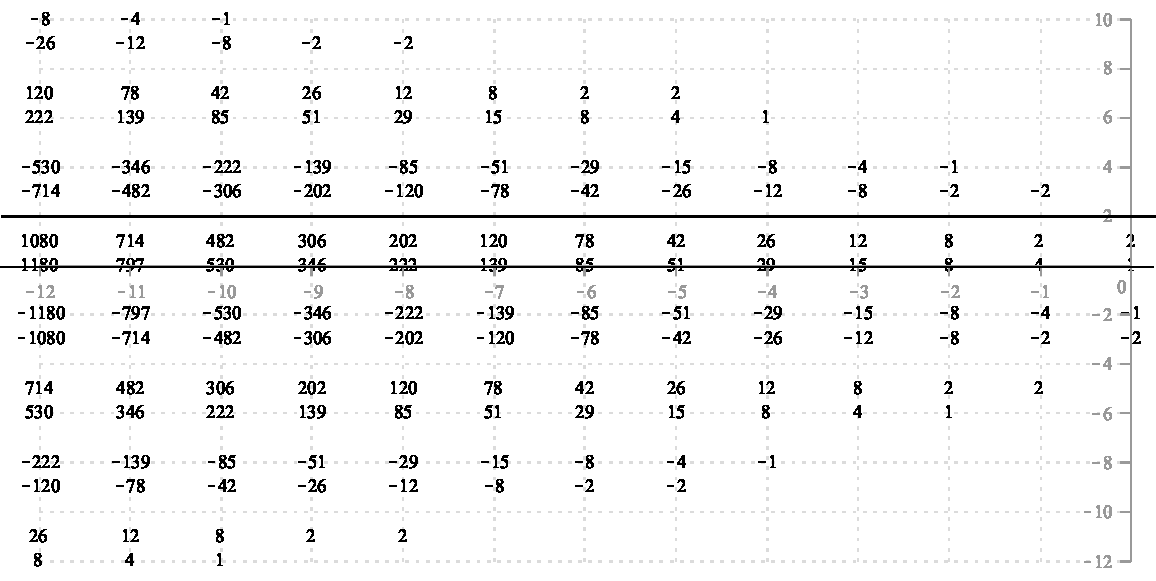
\includegraphics[width=130mm]{AffineB2_A1_branching.pdf}
  \caption{Anomalous branching coefficients for $\hat{A_1}\subset \hat{B_2}$}
  \label{fig:AffineB2_A1_branching}
\end{figure}

Selecting the points inside the main Weyl chamber of the subalgebra $\hat{A_1}$ we get the following results for the branching coefficients up to twelfth grade
\begin{multline}
  \label{eq:28}
  L^{w_1}_{\hat{B_2}\downarrow \hat{A_1}}=2 L_{\hat{A_1}}^{w_1}(0)\oplus 1 L_{\hat{A_1}}^{w_0}(0)\oplus 4 L_{\hat{A_1}}^{w_0}(-1)\oplus\\
    2 L_{\hat{A_1}}^{w_1}(-1)\oplus 8 L_{\hat{A_1}}^{w_0}(-2)\oplus
    8 L_{\hat{A_1}}^{w_1}(-2)\oplus 15 L_{\hat{A_1}}^{w_0}(-3)\oplus\\
    12 L_{\hat{A_1}}^{w_1}(-3)\oplus 26 L_{\hat{A_1}}^{w_1}(-4)\oplus
    29 L_{\hat{A_1}}^{w_0}(-4)\oplus 51 L_{\hat{A_1}}^{w_0}(-5)\oplus\\
    42 L_{\hat{A_1}}^{w_1}(-5)\oplus 78 L_{\hat{A_1}}^{w_1}(-6)\oplus
    85 L_{\hat{A_1}}^{w_0}(-6)\oplus 120 L_{\hat{A_1}}^{w_1}(-7)\oplus\\
    139 L_{\hat{A_1}}^{w_0}(-7)\oplus 202 L_{\hat{A_1}}^{w_1}(-8)\oplus
    222 L_{\hat{A_1}}^{w_0}(-8)\oplus 306 L_{\hat{A_1}}^{w_1}(-9)\oplus\\
    346 L_{\hat{A_1}}^{w_0}(-9)\oplus 530 L_{\hat{A_1}}^{w_0}(-10)\oplus
    482 L_{\hat{A_1}}^{w_1}(-10)\oplus 714 L_{\hat{A_1}}^{w_1}(-11)\oplus\\
    797 L_{\hat{A_1}}^{w_0}(-11)\oplus 1080 L_{\hat{A_1}}^{w_1}(-12)\oplus
    1180 L_{\hat{A_1}}^{w_0}(-12)
\end{multline}
This result can be expressed using the power series expansion of the branching functions \cite{kac1990idl}.
\begin{eqnarray}
  \label{eq:29}
  \begin{array}{cc}
    b^{(w_1)}_{0}= & 1 + 4\,q^{1}+ 8\,q^{2}+ 15\,q^{3}+ 29\,q^{4}+ 51\,q^{5}+ 85\,q^{6}+ 139\,q^{7}+\\
     &222\,q^{8}+ 346\,q^{9}+ 530\,q^{10}+ 797\,q^{11}+ 1180\,q^{12}+\dots\\
  \end{array}\\
  \begin{array}{cc}
    b^{(w_1)}_{1}= &2+2\,q^{1}+8\,q^{2}+12\,q^{3}+26\,q^{4}+42\,q^{5}+78\,q^{6}+120\,q^{7}+\\
    & 202\,q^{8}+306\,q^{9}+482\,q^{10}+714\,q^{11}+1080\,q^{12}+\dots
  \end{array}
\end{eqnarray}
Here the lower index of the branching function denotes the number of the corresponding $\hat{A_1}$ fundamental weight $w_0=\lambda_0=(0,1,0),\; w_1=\alpha/2=(1,1,0)$.


\section{Physical applications}
\label{sec:phys-appl}
Here we want to discuss possible applications of the described techniques in physical models.

Branching coefficients for the embedding of affine Lie subalgebra into
affine Lie algebra can be used to construct modular invariant
partition functions of Wess-Zumino-Novikov-Witten models (\cite{difrancesco1997cft}, \cite{Walton:1999xc}, \cite{walton1989conformal}, \cite{schellekens1986conformal}).

But for this construction to work the embedding is required to be conformal, which means that the central charge of the subalgebra is equal to the central charge of the algebra.
\begin{equation}
  \label{eq:31}
  c(\mathfrak{a})=c(\mathfrak{g})
\end{equation}

 The class of the conformal embeddings is rather small, the complete classification is given in the paper \cite{schellekens1986conformal}.
The requirement (\ref{eq:31}) allows to reduce the task of the computation of the branching coefficients of affine Lie algebras to the computation of the branching coefficients of the finite-dimensional Lie algebras.

Here we describe this procedure and discuss how the requirement (\ref{eq:31}) can be used to simplify the algorithm \ref{sec:algorithm}.

Conformal embeddings should preserve conformal invariance, so Sugawara central charge should be the same for the original and the embedded theory.

The states for the theory that corresponds to the algebra $\mathfrak{g}$
\begin{equation}
  \label{eq:109}
  J^{a_1}_{-n_1}J^{a_2}_{-n_2}\dots\left|\lambda\right>\quad n_1\geq n_2\geq\dots>0
\end{equation}
For sub-algebra $\mathfrak{a}\subset\mathfrak{g}$
\begin{equation}
  \label{eq:110}
  \tilde{J}^{a'_1}_{-n_1}\tilde{J}^{a'_2}_{-n_2}\dots\left|\pi_{\mathfrak{a}}(\lambda)\right>
\end{equation}
Here $\tilde{J}^{a'_j}_{-n_j}$ are the generators of $\mathfrak{a}$ and $\pi_{\mathfrak{a}}$ is the projection of $\mathfrak{g}$ to $\mathfrak{a}$. $\mathfrak{g}$-invariance of vacuum entails its $\mathfrak{a}$-invariance, but it is not the case for energy-momentum tensor. So energy-momentum tensor of bigger theory should consist only of generators of $\mathfrak{a}$. Then $T_{\mathfrak{g}}=T_{\mathfrak{a}}\Rightarrow c(\mathfrak{g})=c(\mathfrak{a})$. This leads to equation
\begin{equation}
  \label{eq:111}
  \frac{k\;\mathrm{dim}\,\mathfrak{g}}{k+g}=\frac{x_e k\; \mathrm{dim}\,\mathfrak{a}}{x_ek+a}
\end{equation}
Here $x_e$ is the embedding index and $g$, $a$ are dual Coxeter numbers of corresponding algebras.

It can be shown that solutions of equation (\ref{eq:111}) exist only
for level 1 $k=1$ \cite{difrancesco1997cft}.

If we have modular-invariant partition function for the fields described by the representation of the algebra $\mathfrak{g}$ this modular invariance is preserved by the projection on the subalgebra $\mathfrak{a}$, but we need also the preservation of the conformal invariance. So we should select only those highest-weight modules of the subalgebra $\mathfrak{a}$ for which the relation (\ref{eq:111}) holds.

Since in the decomposition (\ref{eq:3}) the highest weight $\nu$ of the subalgebra module belongs to some grade $n$ of projected algebra module $\pi_{\mathfrak{a}}\cdot L^{(\mu)}_{\mathfrak{g}}$, from the relation (\ref{eq:111}) one can obtain the following requirement on the conformal dimensions of the corresponding fields
\begin{equation}
  \label{eq:32}
   \Delta_{\pi_{\mathfrak{a}}\mu}+n=\Delta_{\nu}
\end{equation}
It leads to the relation on the classical parts of the corresponding weights:
\begin{equation}
  \label{eq:33}
  \frac{(\overset{\circ }{\mu},\overset{\circ }{\mu}+2\rho)}{2(1+g)}+n=\frac{(\overset{\circ }{\nu},\overset{\circ }{\nu}+2\rho_{\mathfrak{a}})}{2(x_e+a)}
\end{equation}
There exits the finite reducibility theorem for the conformal embeddings which states that only finite number of the branching coefficients is non-zero in the case of the conformal embedding $\mathfrak{a}\subset\mathfrak{a}$.

Then after we have found all such weights $\nu$ and the corresponding branching coefficients $b^{(\mu)}_{\nu}$ we can substitute the sums $\sum_{\nu \in P^{+}_{\mathfrak{a}}}b^{(\mu)}_{\nu} \chi_{\nu}$ over the modified characters $\chi_{\nu}$ of the corresponding $\mathfrak{a}$-modules in place of the characters of the $\mathfrak{g}$-modules in the diagonal modular-invariant partition function
\begin{equation}
  \label{eq:34}
   Z(\tau)=\sum_{ \mu\in P^{+}_{\mathfrak{g}}} \chi_{\mu}(\tau)\bar \chi_{\mu}(\bar \tau)
\end{equation}
Thus we obtain the non-diagonal modular-invariant  partition function for the theory with the current algebra $\mathfrak{a}$.
\begin{equation}
  \label{eq:36}
   Z_{\mathfrak{a}}(\tau)=\sum_{ \nu,\lambda\in P^{+}_{\mathfrak{a}}} \chi_{\nu}(\tau)M_{\nu\lambda}\bar \chi_{\lambda}(\bar \tau)
\end{equation}


\subsection{Example}
\label{sec:example}

\subsubsection{Special embedding $\hat{A}_1\subset\hat{A}_2$}
\label{sec:spec-embedd-hata_1s}
Consider the embedding of the affine Lie algebra $\hat{A}_1$ into $\hat{A}_2$ built as the affine extension of the special embedding $su(2)\subset su(3)$ with the embedding index $x_e=4$. The level of the algebra $\mathfrak{g}=\hat{A}_2$ is equal to one, so the level of the subalgebra $\tilde{k}=kx_e=4$.

There exist three level one dominant weights $[1,0,0],\;[0,1,0],\;[0,0,1]$ in the weight space of $\hat{A}_2$.
It is easy to see that the set $\Delta_{\bot}$ is empty.

Here we view the representation with the highest weight
$w_0=(1,0,0)$ in detail.

The set of the anomalous points of this representation up to sixth grade is depicted in the Figure \ref{fig:affine_A2_anom_point}. We also show the root subspace of the subalgebra $\hat{A}_1$ under consideration.

\begin{figure}[h!tb]
  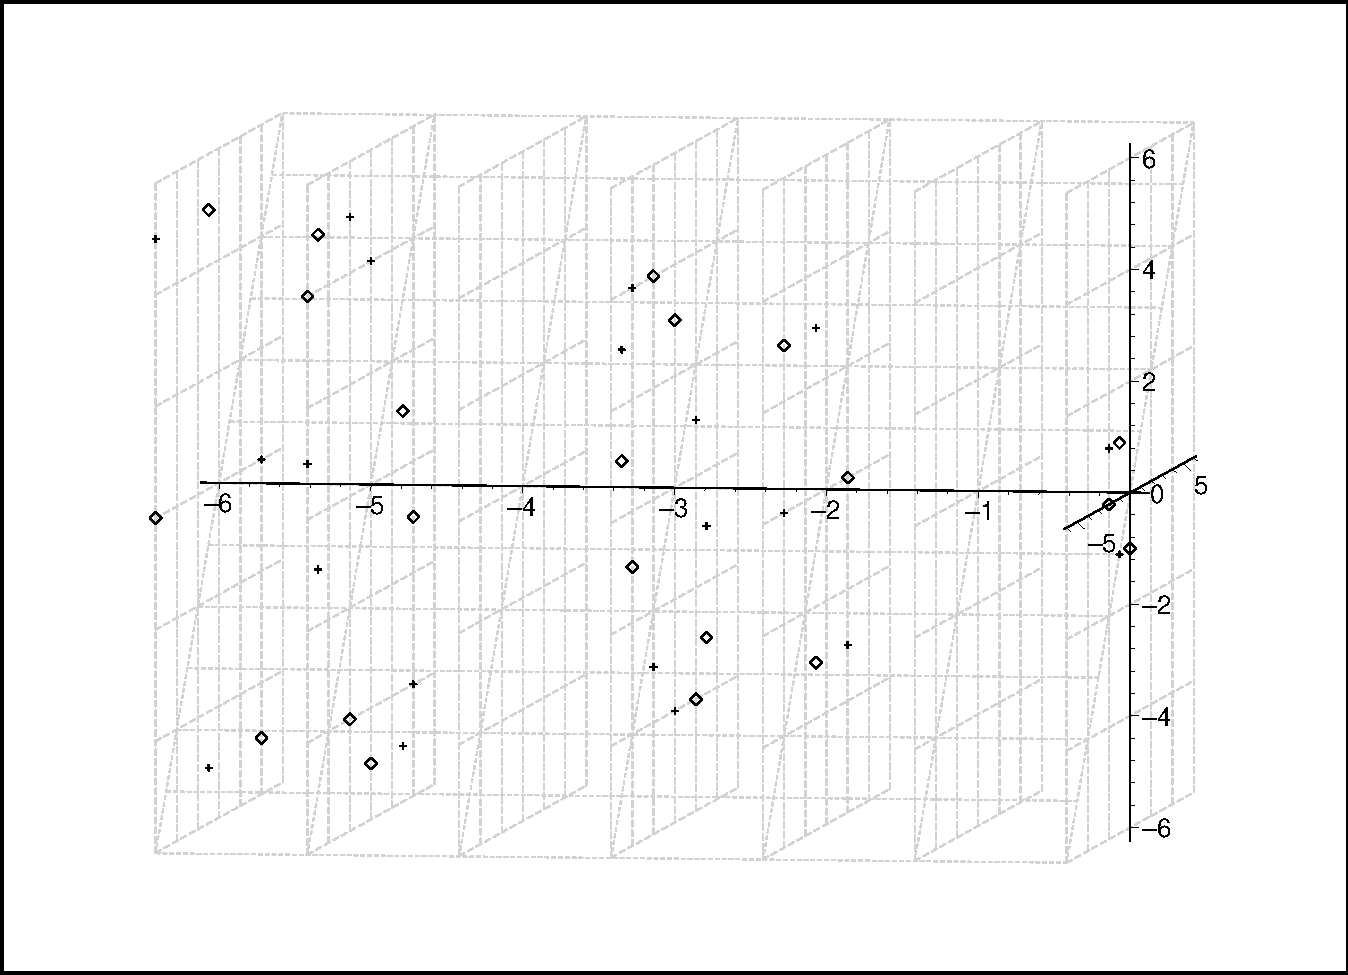
\includegraphics[width=160mm]{AffineA2_A1_anom.pdf}
  \caption{The anomalous points of the $(1,0,1,0)$ representation of the algebra $\hat{A_2}$}
  \label{fig:affine_A2_anom_point}
\end{figure}

As the next step of our algorithm \ref{sec:algorithm} we project the anomalous points to the weight space of the subalgebra $\hat{A_1}$ and calculate the dimensions of the corresponding $\mathfrak{a}_{\bot}$-modules $L^{\pi_{\mathfrak{a}_{\bot}}(\omega(\mu+\rho))-\rho_{\mathfrak{a}_{\bot}}}_{\mathfrak{a}_{\bot}}$.
The result of this computation up to the twelfth grade is presented at the Figure \ref{fig:AffineA2_A1_anom_proj}
\begin{figure}[h!tb]
  \centering
  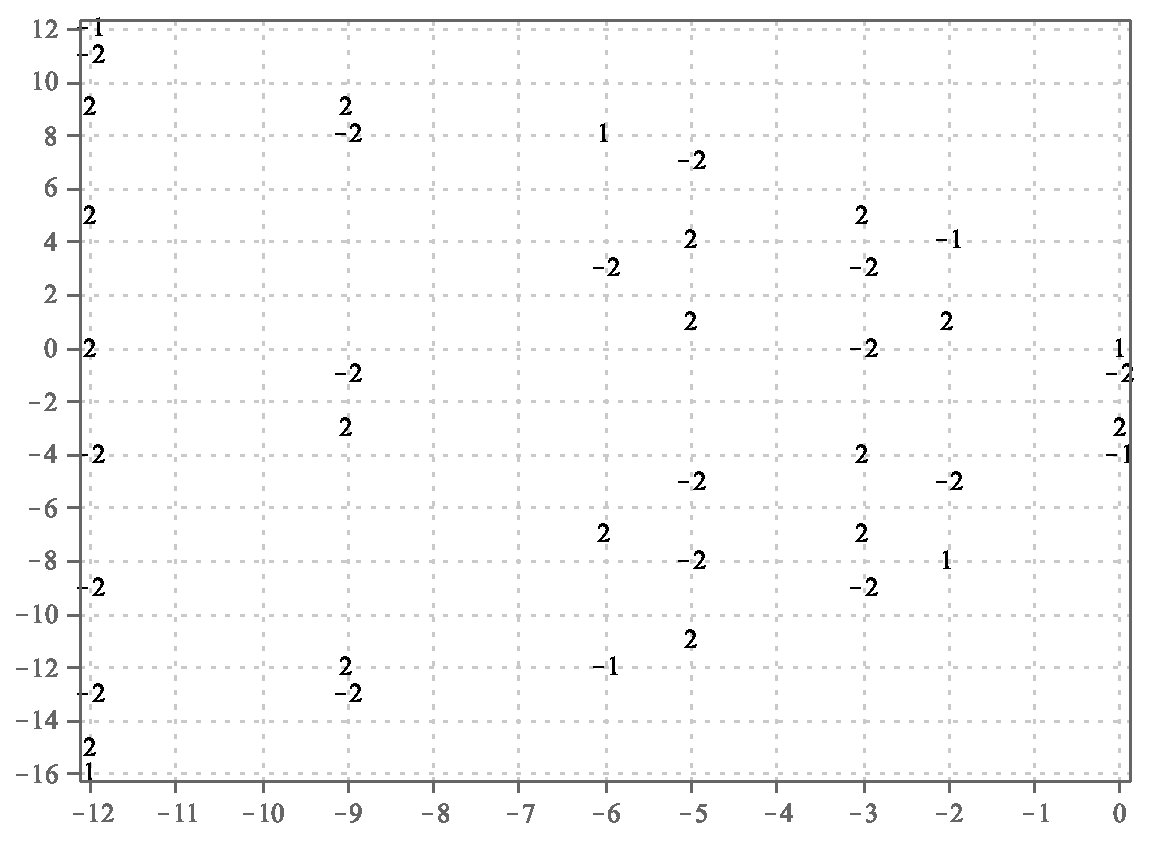
\includegraphics[width=150mm]{AffineA2_A1_proj_anom.pdf}
  \caption{Projected anomalous points and the dimensions of $\mathfrak{a}_{\bot}$-modules.}
  \label{fig:AffineA2_A1_anom_proj}
\end{figure}

Then we should construct ``the fan'' and use the recurrent relation for the computation of anomalous branching coefficients.

Using the definition (\ref{fan-defined}) we get the following set of
the points $\Gamma$ with the corresponding values $s(\gamma+\gamma_0)$, depicted at the Figure \ref{fig:AffineA2A1Fan}.
Here we restricted the computation to the twelfth grade.
\begin{figure}[p]
  \centering
  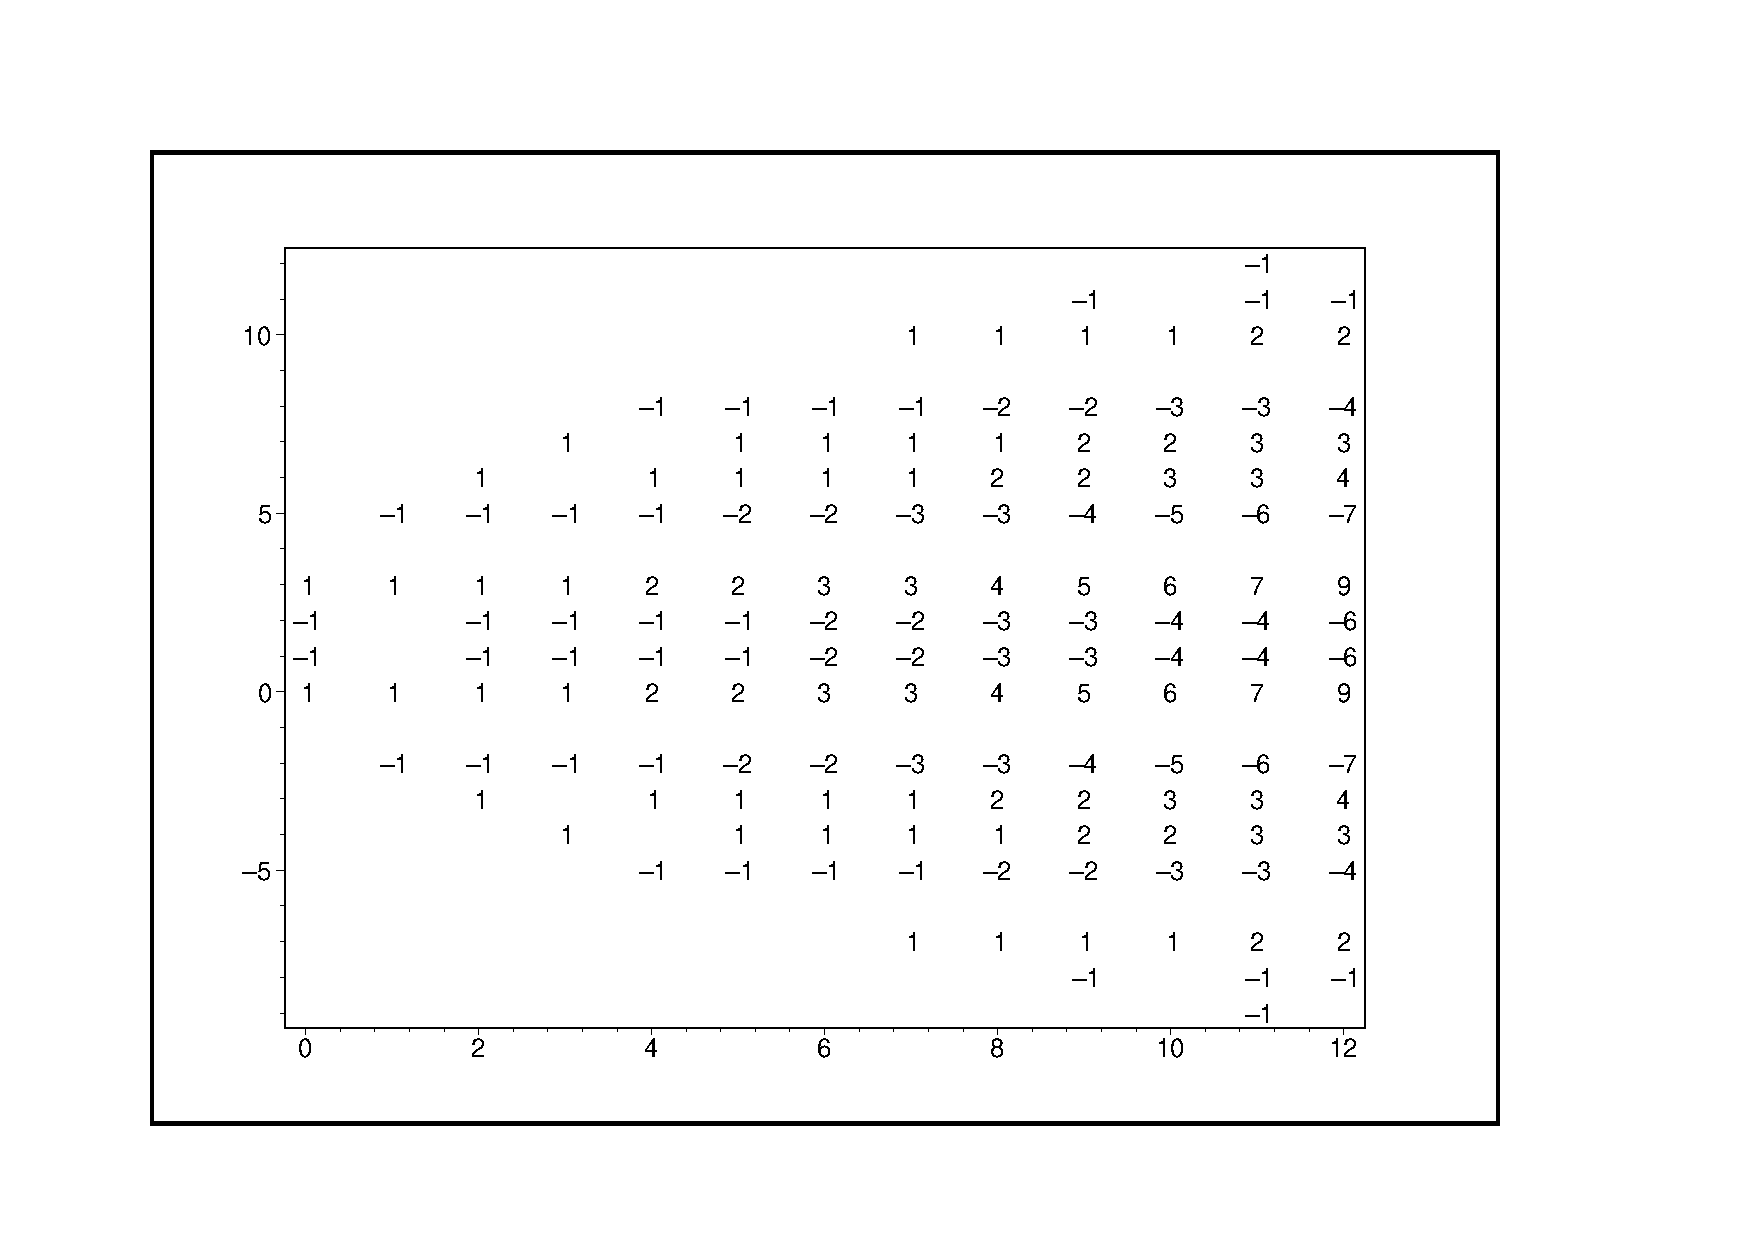
\includegraphics[width=130mm]{AffineA2_A1_fan.pdf}
  \caption{Fan for $\hat{A_1}\subset \hat{A_2}$}
  \label{fig:AffineA2A1Fan}
\end{figure}

Using the recurrent relation for the anomalous branching coefficients we get the following result
\begin{figure}[p]
  \centering
  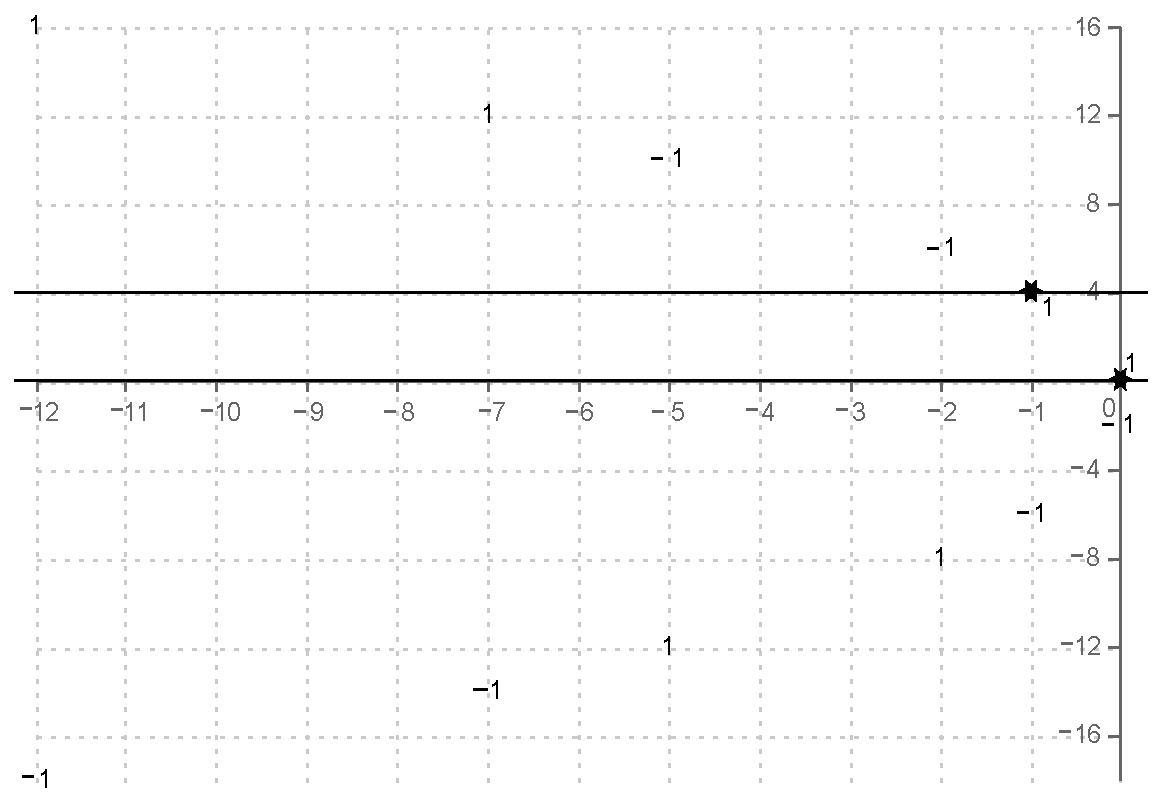
\includegraphics[width=130mm]{AffineA2_A1_branching.pdf}
  \caption{Anomalous branching coefficients for $\hat{A_1}\subset \hat{A_2}$}
  \label{fig:AffineA2_A1_branching}
\end{figure}

We see that only two anomalous branching coefficients inside the main
Weyl chamber of $\hat{A}_1$ are non-zero and equal to the branching
coefficients. So the finite reducibility theorem holds and we get
\begin{equation}
  \label{eq:43}
  L^{[1,0,0]}_{\hat{A_2}\downarrow \hat{A_1}}= L_{\hat{A_1}}^{[0,4]}\oplus L_{\hat{A_1}}^{[4,0]}
\end{equation}

For the other level one dominant weights of $\hat{A}_2$ we get trivial
branching rules
\begin{eqnarray}
  \label{eq:44}
   L^{[0,1,0]}_{\hat{A_2}\downarrow \hat{A_1}}= L_{\hat{A_1}}^{[2,2]}\\
   L^{[0,0,1]}_{\hat{A_2}\downarrow \hat{A_1}}= L_{\hat{A_1}}^{[2,2]}
\end{eqnarray}

Using this result we can construct modular-invariant partition function
\begin{equation}
  \label{eq:45}
  Z=\left|\chi_{[4,0]}+\chi_{[0,4]}\right|^2+2\chi_{[2,2]}^2
\end{equation}

\section{Conclusion}
\label{sec:conclusion}
We have constructed the recurrent relation for branching coefficients and proposed practical algorithm for the reduction procedure. Also we have discussed the application of this algorithm to the physical problem of construction the modular-invariant partition functions in the conformal field theory. This method of conformal embeddings is well-known but may be actual in the study of WZW-models emerging in the context of the AdS/CFT correspondence \cite{Maldacena:2000hw,Maldacena:2000kv,Maldacena:2001km}.


\section{Acknowledgements}
The work was supported in
part by RFFI grant N 09-01-00504 and the National Project RNP.2.1.1./1575.

\bibliography{article}{}
\bibliographystyle{utphys}

\end{document}
